% gjilguid2e.tex
% V2.0 released 1998 December 18
% V2.1 released 2003 October 7 -- Gregor Hutton, updated the web address for the style files.

\documentclass{gji}
\usepackage{timet,color}
\usepackage[urlcolor=blue,citecolor=black,linkcolor=black,colorlinks=True,breaklinks=True]{hyperref}
\urlstyle{same}
\usepackage[authoryear]{natbib}
\usepackage{multirow}
\usepackage{multicol}
\usepackage{booktabs}
\usepackage{threeparttable}
\usepackage{graphicx}
%\usepackage{lineno}
%\linenumbers
%\renewcommand\linenumberfont{\normalfont\bfseries\small}
\graphicspath{{./figures/}}
\def\refname{REFERENCES}

\title[Seismic source discrimination]
  {Deep learning and transfer learning of earthquake and quarry-blast discrimination: Applications to southern California and eastern Kentucky}
\author[J. Zhu \emph{et al.}]
  {Jun Zhu,$^1$ Lihua Fang,$^2$ Fajun Miao,$^3$ Liping Fan,$^2$ Ji Zhang$^1$ and Zefeng Li$^{1,4*}$ \\
  $^1$ Laboratory of Seismology and Physics of Earth’s Interior, School of Earth and Space Science,\\University of Science and Technology of China, \emph{230026}, Hefei, China. E-mail: \href{mailto:zefengli@ustc.edu.cn}{zefengli@ustc.edu.cn}\\
  $^2$ Institute of Geophysics, China Earthquake Administration, \emph{100081}, Beijing, China\\
  $^3$ Jiangsu Earthquake Administration, China Earthquake Administration, \emph{210014}, Nanjing, China\\
  $^4$ Mengcheng National Geophysical Observatory, University of Science and Technology of China, \emph{233500},\\Mengcheng, China}
\date{Accepted 2023 November 22. Received 2023 October 13; in original form 2023 February 13}
\pagerange{\pageref{firstpage}--\pageref{lastpage}}
\volume{200}
\pubyear{2023}

%\def\LaTeX{L\kern-.36em\raise.3ex\hbox{{\small A}}\kern-.15em
%    T\kern-.1667em\lower.7ex\hbox{E}\kern-.125emX}
%\def\LATeX{L\kern-.36em\raise.3ex\hbox{{\Large A}}\kern-.15em
%    T\kern-.1667em\lower.7ex\hbox{E}\kern-.125emX}
% Authors with AMS fonts and mssymb.tex can comment out the following
% line to get the correct symbol for Geophysical Journal International.
\let\leqslant=\leq

\newtheorem{theorem}{Theorem}[section]

\begin{document}

\label{firstpage}

\maketitle


\begin{summary}
Discrimination between tectonic earthquakes and quarry blasts is important for accurate earthquake cataloguing and seismic hazard analysis. However, reliable classification of these two types of seismic events is challenging with no prior knowledge of source parameters. Here we applied deep learning to perform this classification task in southern California and eastern Kentucky. Since the two regions differ significantly in available labelled data, class imbalance and waveform characteristics, we adopted different strategies for them. We directly trained a convolutional neural network (CNN) for southern California due to its data abundancy. To alleviate the class imbalance, the blast data were augmented by repeated sampling. The model for California yields F1-scores of \textgreater{83.5}\% when estimated by individual stations and \textgreater{98.1}\% by network average (i.e., averaging the CNN's outputs on all available stations for each event). As eastern Kentucky has a much smaller data size, we apply transfer learning to the pretrained California model to fit the Kentucky data. The transfer-learned model yields F1-scores of \textgreater{86.9}\% when estimated by individual stations and \textgreater{96.7}\% by network average. The transfer-learned model outperforms the model re-trained from scratch for the Kentucky data. Gradient-weighted class activation mapping shows the \textit{S} onset and the \textit{S} long-period coda are important to identify earthquakes and blasts, respectively. By visual inspections of the seismograms, the source locations, the origin time and the \textit{P}-wave polarities, we verified that most of the events falsely predicted by our models are actually mislabelled by seismic analysts. Our models thus show great potential in helping seismic analysts find those mislabelled events which remain hidden in the historical catalogue. Our results demonstrate that deep learning can achieve high accuracy in seismic event discrimination and that transfer learning is effective and efficient to generalize deep learning models across different regions.
\end{summary}

\begin{keywords}
Seismicity and tectonics; Neural networks, fuzzy logic; Controlled source seismology; Earthquake source observations
\end{keywords}

\section{Introduction}
Modern seismic networks have improved considerably over the past decades and have increasingly recorded diverse seismic signals other than earthquakes. These signals have natural origins such as landslides and debris flows, or anthropogenic origins such as industry exploitation blasts and traffic flow. On one hand, discrimination between local tectonic earthquakes (EQs) and other seismic signals is important for seismic hazard analysis. Recent studies show that seismic catalogues contaminated by quarry blasts (QBs) can result in an overestimated b-value and thus an underestimated probability of large earthquakes \citep{tang,gulia_19,gulia_21}. On the other hand, classification of these signals can provide valuable resources in environmental seismology \citep{larose}, urban seismology \citep{diaz} and forensic seismology \citep{douglas}. For example, in mining areas, monitoring blasting events with small magnitudes has practical uses for supervising safe production and detecting illegal mining activities \citep{illegal,illegal_book}. Either to clean up earthquake catalogues or to construct catalogues of non-earthquake events, interest in classifying different types of events has grown rapidly over the past years.

Discrimination between earthquakes and quarry blasts has been a challenging task in seismic network operation for a long time owing to their apparent similarity in waveform characteristics. Seismologists have proposed a variety of automated approaches, which can be roughly divided into two categories: source-parameter-based and waveform-based. The former relies on source information like location and\slash or origin time \citep{fereidoni,wiemer,semiautomated}. For example, blasts tend to cluster in known quarry sites with shallow depths (\textless{2} km) and occur almost entirely in the daytime. However, source location information requires accurate preceding analyses, limiting its application in real-time processing. Comparatively, waveform-based approaches use seismic waveform features only, either defined by experienced experts or automatically extracted from data, or a combination of both \citep{allmann,wang_jgr,wang_grl,koper,koper_20,hartse,korrat,linville_19,miao,su,tibi_depth,tibi_compare,kong}.

Manually defined features include spectral ratios of \textit{Lg} \citep{bennett} and \textit{Rg} \citep{tibi_depth}, \textit{P}-to-\textit{S} phase ratios \citep{hartse,wang_grl,wang_jgr,kong}, $M_L$-$M_C$ \citep[$M_L$, local magnitude; $M_C$, coda magnitude.][]{koper,koper_20,wang_grl,kong}, the misfit of \textit{P}-wave spectra to an $\omega^{-2}$ source model \citep{allmann} and multiwindow frequency contents \citep{miao}. In particular, blast signals tend to have emergent \textit{P}-waves and weak \textit{S}-waves, upward \textit{P}-wave polarities and Gaussian-like envelopes, whereas earthquake signals often have clear \textit{P}- and \textit{S}-waves \citep{miao,stump,tang}. Generally, the performance of waveform-based approaches depends on the generalizability of the extracted features. Features crafted for one region may be unsuitable for another so that the classification performance could drop significantly. Moreover, waveform features cannot be reliably measured in presence of high noise and thus small events could be difficult to classify \citep{linville_19,tibi_compare}.

Instead of using manually defined features, deep learning enables direct extraction of implicit features from data \citep{linville_19,liu,gpd,polarity,zhulijun,phasenet}. The features are sought greedily during the training process that maps the input waveforms to the output class. Thereby, they are likely more representative than manually-defined features. However, deep learning models contain a large number of parameters and thus require large sets of high-quality labelled data to avoid overfitting (i.e., the model memorizes the data rather than learns the generalizable rules). Such data sets may not always be available, especially in areas with a short monitoring history, a low seismic activity level, or lack of manual labels. In this case, transfer learning could be helpful as it leverages the knowledge learned from a rich dataset and applies to another dataset with minor modifications \citep{chai,do,ismail,pan_domain,zhuy,transferable}. With a well-trained base model, transfer learning only takes a small number of labels to adequately fine-tune the model.

In this study, we built a deep learning model to discriminate events in southern California by using a large number of labelled earthquakes and blasts, and on this basis applied transfer learning to build another model for eastern Kentucky. We adopted different strategies for the two regions because eastern Kentucky has limited earthquake examples. Moreover, we implemented data augmentation to mitigate the effect of class imbalance in the two regions. The southern California model achieves an accuracy of 95.3\%, an F1-score of 97.3\% for earthquakes and 83.5\% for blasts. The transfer-learned model to eastern Kentucky achieves an accuracy of 99.0\%, an F1-score of 86.9\% for earthquakes and 99.5\% for blasts. In both cases, the smaller class (blasts in southern California, earthquakes in eastern Kentucky) tends to have a lower precision and F1-score. Both the California and the Kentucky model yield an F1-score of \textgreater{83.5\%} for the smaller class. We implemented gradient-weighted class activation mapping \citep[Grad-CAM,][]{cam} to investigate which parts of the waveforms are important for decision making. Finally, we discuss the advantages and practical considerations of our models and offer suggestions for further use of them.

\section{Data}
\subsection{Southern California}
Southern California is instrumented by the Southern California Seismic Network \citep[SCSN,][]{scsn} with a long earthquake monitoring history since 1932. The event types catalogued in SCSN include tectonic earthquakes, quarry blasts, sonic booms, nuclear blasts and unknown types. In this study we kept one of every six tectonic earthquakes in the SCSN catalogues from 2011 to 2020 to mitigate data imbalance, and ultimately obtain 37,727 local earthquakes and 6,702 blasts (Fig.~\ref{map}) recorded by 337 seismic stations (Fig.~S1). We limit the maximum epicentral distance to 100 km in southern California because of the generally high SNR (signal-to-noise ratio, defined by eq.~\ref{snr}) and sufficient station coverage within this distance. The aftershocks of the 2019 Ridgecrest earthquake have been removed to avoid potential bias. This results in a total of 1,721,092 three-component earthquake recordings and 312,911 blast recordings, a class ratio approximately 5.5:1. We describe the data augmentation procedure used to improve the class balance in the method section.

All the waveforms are sampled at 100 Hz and recorded by high gain seismometers with a channel code HH[E\textbar{N}\textbar{Z}]. They were preprocessed as follows. First, the waveforms were detrended, tapered with a Hanning window and globally normalized by the maximal standard deviation of three components. Second, we picked \textit{P}-wave arrivals by searching the PhaseNet \textit{P}-picks \citep{phasenet} within 3 s around theoretical arrivals (Fig.~\ref{phasenet}). We apply the PhaseNet model \citep{phasenet} to pick \textit{P}-arrivals. The theoretical arrival prediction used the Hadley-Kanamori 1D velocity model \citep{kanamori,hadley}. We use PhaseNet picks because they are much more abundant than the SCSN picks. The data quality is ensured by the following criteria: We only used the PhaseNet \textit{P}-picks within $\pm{3}$ s of the theoretical arrival time, with an SNR \textgreater{0} dB, and a PhaseNet probability \textgreater{0.3}.
We use a relatively low SNR threshold because of the follwing reasons: 1) PhaseNet can produce relatively reliable picks above the preset threshold, with a precision of 0.85 for SNR \textless{0} dB picks \citep[fig.~8a in][]{phasenet}; 2) We require the PhaseNet \textit{P}-pick to be near the \textit{P}-wave arrival predicted by the 1D southern California velocity model \citep{hadley,kanamori}. This serves as another screener for data quality; 3) The low SNR waveforms can help improve the model robustness in presence of noise during training. Third, we applied a 1-15 Hz bandpass filter to all the recordings. We chose the 1-15 Hz frequency band due to its dominance over the energy of local seismicity \citep{allmann}. Finally, the waveforms are cut 5 s before and 55 s after the first arrival. After applying the SNR threshold, the resulting data set contains 29,075 -0.48\textless{$M_L$}\textless{5.51} earthquakes (583,706 recordings) and 6,632 0.17\textless{$M_L$}\textless{2.56} blasts (77,707 recordings). Fig.~S2 shows the histograms of magnitude, depth, epicentral distance and SNR for this data set.

\begin{figure*}
\centering
\includegraphics[width=.99\textwidth]{event.pdf}
\caption{Distribution of local earthquakes (red dots) and quarry blasts (blue dots) in the California data set. The bottom left inset shows the statistics of 29,075 natural earthquakes and 6,632 quarry blasts, whose SNR are \textgreater{0} dB. The top left inset marks the study area. The red and the blue star mark an earthquake (SCEDC event ID 38613378) and a blast (39363607) potentially mislabelled by SCSN analysts, respectively. Fig.~\ref{mislabel} shows the corresponding waveforms.}
\label{map}
\end{figure*}

\begin{figure}
\centering
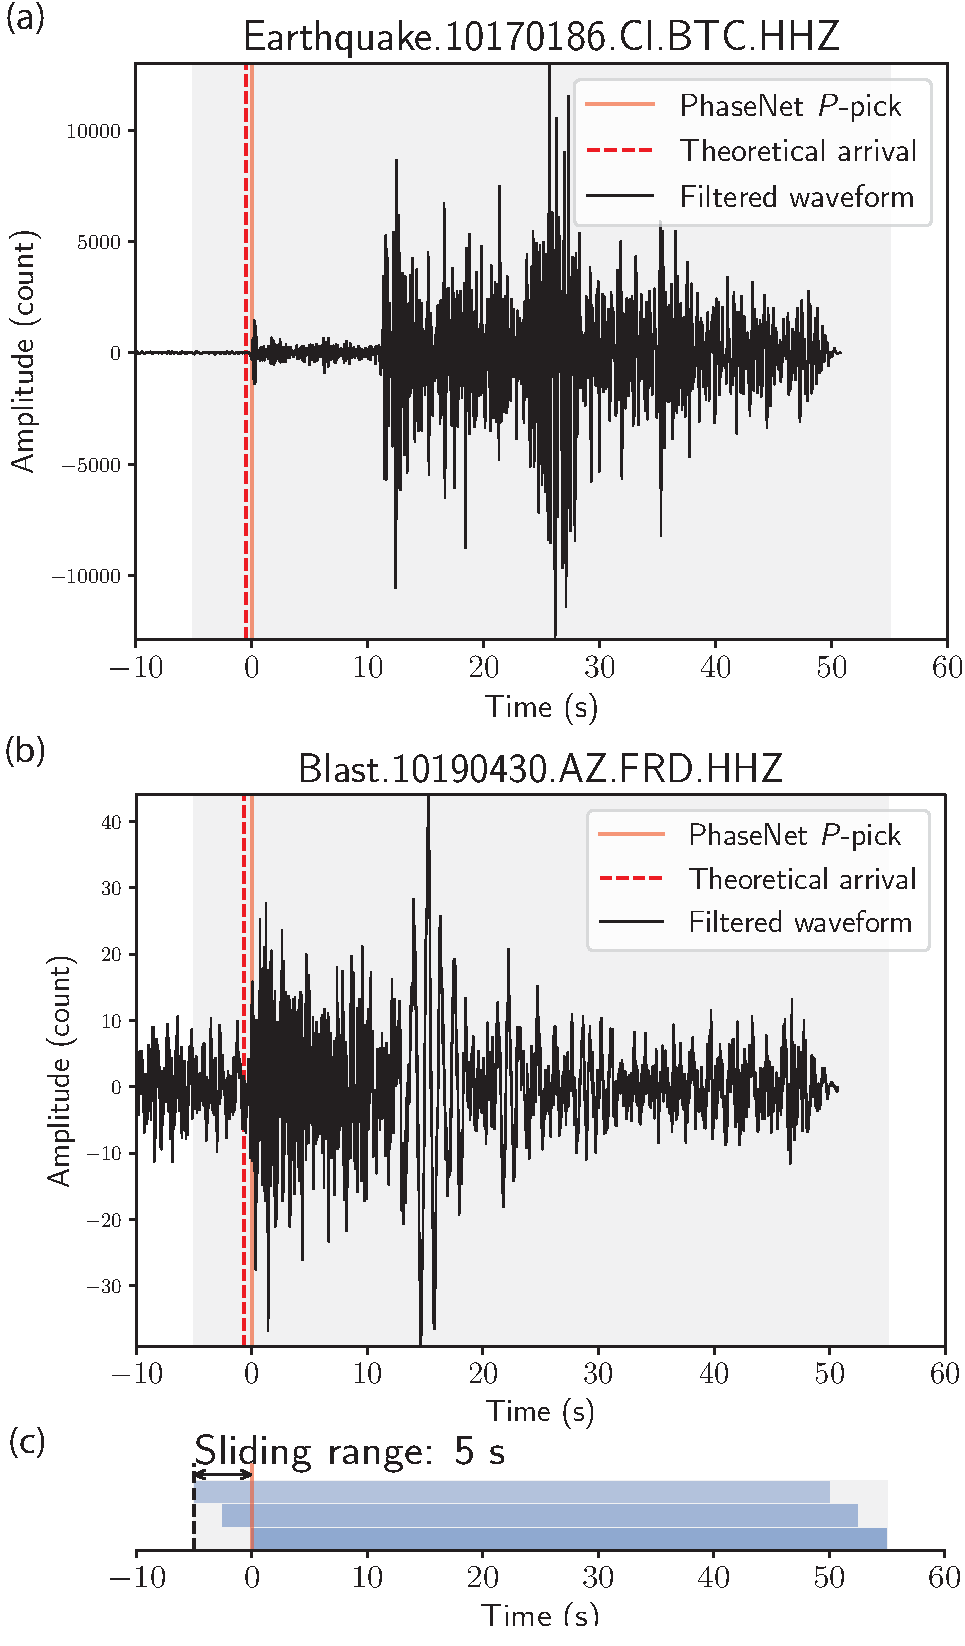
\includegraphics[width=.48\textwidth]{window.pdf}
\caption{Example model inputs: (a) earthquake and (b) blast waveform windowed by (c). The red dashed and the red solid line mark the theoretical \textit{P}-wave arrival time and the \textit{P}-pick predicted by PhaseNet \citep{phasenet}, respectively. The last parts of these two recordings are empty because the data we downloaded are triggered rather than continuous waveforms. The empty parts will be filled with zeros when fed into the model. The input waveform has a duration of 55 s, i.e., the blue rectangles in (c). The start of the input is allowed to shift within the 5 s (black arrow) before the PhaseNet pick during training.}
\label{phasenet}
\end{figure}

\begin{figure}
\centering
\includegraphics[width=.48\textwidth]{event_ek.pdf}
\caption{Distribution of local earthquakes and quarry blasts in the Kentucky data set. Symbols are the same as Fig.~\ref{map}. We highlight Event 1 (red star) and 2 (blue star) as they are the only two predictions disagreeing with true labels (i.e., the only two mispredictions). Fig.~\ref{mislabel_ek} shows the corresponding waveforms.}
\label{map_ek}
\end{figure}

\subsection{Eastern Kentucky}
Another dataset is from \cite{miao} who compiled waveforms of earthquakes and blasts in eastern Kentucky. It contains 150 natural earthquakes (2,091 recordings) and 4,218 quarry blasts (56,643 recordings) from June 2015 to March 2019 (Fig.~\ref{map_ek}), recorded by 35 regional seismic stations and a temporary network EKMMP of 13 seismic stations (Fig.~S3). These events were detected by coincidence triggering on \textgreater{3} stations, using the Earthworm software package (see Data Availability). They were manually classified as earthquake or blast by \cite{miao}. The \textit{P} and \textit{S} arrivals were picked and linked to the triggered events also by \cite{miao}, using generalized phase detection \citep[GPD,][]{gpd} and PhasePAPy \citep{phasepapy}, respectively. As this dataset is relatively small, we kept all the instrument types (EH*, BH* and HH*) but resampled all of them to 100 Hz. Other preprocessing steps are similar to those for the California data set. Fig.~S4 shows the histograms of magnitude, depth, epicentral distance, and SNR for the Kentucky data set. The magnitude and depth of the blasts are not available \citep{miao}.

The eastern Kentucky data set differs from the California one in data size and class balance. Eastern Kentucky is relatively quiet in seismicity and has frequent quarry blasts due to prosperous mining industry in the region \citep{carpenter}. In addition, most events in Kentucky have an epicentral distance longer than 100 km due to relatively sparse seismic networks, compared to the shorter epicentral distance and denser seismic networks in southern California. The differences in the two datasets provide an opportunity to test the effectiveness of transfer learning across two separate regions.
\begin{table*}
\caption{Data division}
\label{division}
\begin{threeparttable}[b]
    \begin{tabular}{cccccc}
    \toprule[1pt]
    Region & Split ratio & Type$^a$  & Time span & Recordings & Events \\
    \midrule
    \multirow{6}[2]{*}{California$^b$} & \multirow{2}[1]{*}{70\% for training} & EQ    & Jan. 2011 - Sept. 2018 & 384,695 & 20,353 \\
          &       & QB    & Jan. 2011 - Jan. 2018 & 47,925 & 4,643 \\
          & \multirow{2}[0]{*}{10\% for validation} & EQ    & Sept. 2018 - Jul. 2019 & 65,438 & 2,907 \\
          &       & QB    & Jan. 2018 - Dec. 2018 & 9,284 & 663 \\
          & \multirow{2}[1]{*}{20\% for test} & EQ    & Jul. 2019 - Dec. 2020 & 133,573 & 5,815 \\
          &       & QB    & Dec. 2018 - Dec.2020 & 20,498 & 1,326 \\
    \midrule
    \multirow{6}[2]{*}{Kentucky} & \multirow{2}[1]{*}{70\% for training} & EQ    &  Jun. 2015 - Oct. 2017 & 1,411 & 105 \\
          &       & QB    &  Jun. 2015 - Sept. 2017 & 39,503 & 2,952 \\
          & \multirow{2}[0]{*}{10\% for validation} & EQ    &  Oct. 2017 - Jan. 2018 & 200   & 15 \\
          &       & QB    & Sept. 2017 - Jan. 2018 & 5,543 & 421 \\
          & \multirow{2}[1]{*}{20\% for test} & EQ    & Jan. 2018 - Mar. 2019 & 446   & 30 \\
          &       & QB    & Jan. 2018 - Dec. 2018 & 11,515 & 845 \\
    \bottomrule[1pt]
    \end{tabular}%
     \begin{tablenotes}
     \item[$a$] EQ, natural earthquake; QB, quarry blast;
     \item[$b$] The aftershocks of the 2019 Ridgecrest earthquake have been removed.
   \end{tablenotes}
\end{threeparttable}
\end{table*}
\section{Methods}
\subsection{Data division and augmentation}
We used the same data splitting strategy for the two regions. For example, the southern California dataset was divided into three subsets: training (70\%), validation (10\%) and test set (20\%). To avoid data leakage (i.e., the model training uses information that is unavailable in real-world applications), we split the dataset at the event level, i.e., recordings from the same event were allocated to the same subset. To mimic the scenario of near real-time classification, the events in the training, validation and test sets were split chronologically (Table~\ref{division}) as recommended by \cite{linville_19}. This practice allows assessing model performances under more realistic monitoring conditions.

As local earthquakes are predominant in the southern California dataset, the trained model tends to capture more characteristics of and thus have better identification of earthquakes than blasts. This tendency stems from the fact that the majority class dominates the weight update process of model training \citep{imbalance}. Hence, data augmentation is needed to increase both the quantity and the diversity of the training set, especially for the quarry blasts. We randomly shifted the start of the 55-s time window of model input to create multiple copies of quarry blasts (Figs.~\ref{phasenet}b and \ref{phasenet}c). We took 5 random shifts for recordings of quarry blasts (hence repeated sampling quarry blasts for 5 times) and only 1 random shift for recordings of local earthquakes. Conversely, to balance the two classes in the eastern Kentucky dataset, we augmented the number of earthquakes by 16 random shifts and kept 1 random shift for quarry blasts. We have also tried other random shifts (1, 2, 4, 8, and 27) for the earthquakes in Kentucky and found 16 shifts produces optimal and stable results. In addition to repeated sampling, four basic seismic data augmentation techniques were used to expand both types of events (Appendix~\ref{data_aug}).

For the California case, we have tried two other strategies to mitigate the effects of the extreme class imbalance: downsampling earthquakes and cost-sensitive learning \citep{cost_sensitive}. We will compare their performances and comment on their pros and cons in the discussion section.

\begin{figure*}
\centering
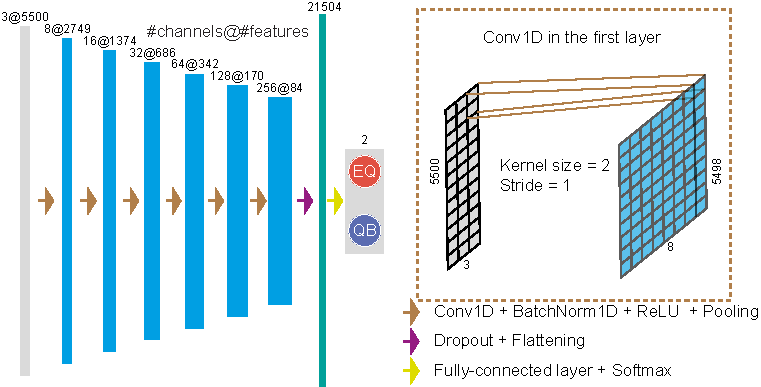
\includegraphics[width=.99\textwidth]{CNN6.pdf}
\caption{The architecture of the convolutional neural network (CNN, left). The CNN model consists of six convolutional layers (brown, each including four basic operations: 1D-convolution, batch normalization, the ReLU activation function and max pooling), one dropout (purple) and one fully connected layer (yellow). The rectangles represent the model input and each layer’s output, with their dimensions and functions annotated by the numbers and colours, respectively. The 1D-convolution operation in the first layer is shown in the brown box.}
\label{cnn6}
\end{figure*}

\subsection{Deep learning: the CNN architecture}
CNNs essentially learn a nonlinear function that maps 2-D images or 1-D time-series data to class labels \citep{lecun}. Compared with a multilayer perceptron, a CNN introduces a feature extractor which consists of several convolutional layers. Each layer receives the locally connected input from its previous layer. After convolving the input with a filter (convolutional kernel), the layer subsamples the output and sends it to the subsequent layer at the locally connected position. The convolutional kernels are determined during the training process to parameterize the general object features. As these kernels are shared across a layer and convolutional downsampling is done through the model, the feature extractor is generally insensitive to specific locations and scales of the salient features. Since 2018, CNNs have been widely applied to seismic data processing, such as earthquake detection \citep{perol}, phase picking \citep{gpd,zhulijun,phasenet}, first-motion polarity identification \citep{polarity} and seismic source discrimination \citep{linville_19,liu,tibi_compare,kong}. Especially, CNNs were proposed to distinguish between earthquakes and quarry blasts in Utah with spectrograms as input \citep{linville_19,tibi_compare}.

We designed a new CNN model (Fig.~\ref{cnn6}) to discriminate earthquakes and blasts in southern California using 55 s three-component waveforms (dimension [3, 5500]). The 55 s window is sufficiently long to include the major phases as well as the coda in both California and Kentucky. The model contains six convolutional layers (the brown box in Fig.~\ref{cnn6}), one dropout and one fully-connected layer. A Rectified Linear Unit (ReLU) nonlinear activation function is used in each convolutional layer. Each convolutional layer is followed with a batch normalization and a max pooling layer. In the bottom, a fully-connected layer, together with a dropout layer, serves as a downstream classifier. The dropout layer designed to avoid overfitting \citep{dropout} has a dropout rate of 0.3. The final output is a two-node probability vector representing the likelihoods of an earthquake and a blast, respectively. We added a softmax activation function in the last layer so that the values of the two nodes are non-negative and summed to be 1.

The CNN model has a total of 131,866 trainable parameters and is built on the PyTorch framework \citep{torch}. Similarly, to avoid overfitting, we ended training when the loss on validation set fails to decrease over five epochs and saved the model with the lowest validation loss, a common training strategy called early stopping in deep learning \citep{early_stop}. The training was completed after 15 epochs on a workstation with Nvidia Graph Process Unit A100-PCIE-40GB, approximately 19 hours. In this study, hyperparameters (i.e., predefined training parameters, Table S1) are shared by all the models, except for the transferred Kentucky models which have a smaller learning rate and will be introduced in the next section.

\subsection{Transfer learning: fine-tuning/freezing the pretrained model}
\label{transfer_learning_strategy}
A deep learning model typically contains tens of thousands to millions of parameters to be determined during the training process. Sufficient data thus are needed to constrain them without overfitting. As previously mentioned, the California model contains 131,866 parameters and is trained on 661,413 recordings. In comparison, the Kentucky data have only 58,734 recordings, an order of magnitude less. Moreover, the Kentucky data have more quarry blasts than earthquakes, which is the opposite of the class balance in southern California. Furthermore, the epicentral distance is generally longer in Kentucky (Fig.~S4c). Finally, the differences in seismic attenuation \citep{attenu_ek,attenu_socal} and velocity structures of southern California and eastern Kentucky could lead to differences in the recorded earthquake and blast waveforms. Therefore, direct application of the California model to Kentucky could be unsatisfactory and model modification is required.

Transfer learning provides a convenient tool to modify deep learning models. Typically, deep learning models hypothesize that the training data are independent and identically distributed with the test data; transfer learning relaxes this hypothesis to extend the applications to similar tasks \citep{tan}. Transfer learning has been proved to be efficient and effective in many other fields \citep{long,long_15,pan_domain}, whereas its applications in seismology are rather limited. As an early example, \cite{zhulijun} trained a phase picker on the 2008 $M_W$7.9 Wenchuan earthquake sequence and fine-tuned it for an Oklahoma data set. By modifying the PhaseNet model, which was learned from regional seismic networks \citep{phasenet}, \cite{chai} made it work well for microseismic data with a much higher sampling rate and a smaller data size than those for training the original PhaseNet. They reported that the transfer-learned model outperforms both the original PhaseNet and even human analysts.

In practice, fine-tuning a deep learning model is straightforward. Instead of re-training the model from scratch where the model parameters are randomly initialized, transfer learning uses the original model as a starting point and continues to train the model with new data. Alternatively, one can freeze parameters of the shallow submodules of the original model and only modify the rest. The fine-tuning with freezing (called freezing hereafter) is useful when the training set is small and shares a similar data distribution with that of the pretrained model. Both the fine-tuning and the freezing strategy fine-tune the model. The difference lies in that the former updates the whole network while the latter updates only the deepest layer(s) within the network. Both strategies were tested and their performances will be compared in the next section.

\section{Results}

\subsection{Deep learning for southern California}
For each seismogram, the model outputs two probabilities corresponding to the likelihood of each class. If the probability for natural earthquakes is above a threshold of 0.5, the seismogram is assigned to the earthquake class, otherwise the blast class. As an event is often recorded by multiple stations, more reliable classification is achieved by averaging over the stations with \textit{P}-wave SNR above 0 dB. We evaluated the classification performance quantitatively with confusion matrices at both the station level (individual recordings) and the network level (network average). To describe the performance in the framework of typical classification tasks, we defined blasts as positive predictions and earthquakes as negative predictions. Following this definition, a confusion matrix consists of four elements:
\begin{enumerate}
\renewcommand{\theenumi}{(\arabic{enumi})}
\item True positive (TP): blasts predicted as blasts;
\item True negative (TN): earthquakes predicted as earthquakes;
\item False positive (FP): earthquakes predicted as blasts;
\item False negative (FN): blasts predicted as earthquakes.
\end{enumerate}

\begin{equation}
\label{recall}
R_{EQ}=\frac{TN}{TN+FP},\\R_{QB}=\frac{TP}{TP+FN}
\end{equation}
\begin{equation}
\label{precision}
P_{EQ}=\frac{TN}{TN+FN},\\P_{QB}=\frac{TP}{TP+FP}
\end{equation}
\begin{equation}
\label{F1}
F1_{EQ}=\frac{2 \cdot R_{EQ} \cdot P_{EQ}}{R_{EQ}+P_{EQ}},\\F1_{QB}=\frac{2 \cdot R_{QB} \cdot P_{QB}}{R_{QB}+P_{QB}}
\end{equation}
\begin{equation}
\label{acc}
Acc=\frac{TP+TN}{TP+TN+FP+FN}
\end{equation}

We further defined recall as fraction of true samples that are correctly classified (eq.~\ref{recall}), and precision as fraction of classified samples that are true samples (eq.~\ref{precision}). In addition, we defined F1-score as the harmonic mean of precision and recall (eq.~\ref{F1}), and accuracy as the fraction of predictions that are correct (eq.~\ref{acc}). We argue that the F1-score is unbiased compared to other evaluation metrics (e.g., the accuracy which is susceptible to model's performance on the majority class).

Table~\ref{socal_performance} and Fig.~\ref{histogram}a show that most of the test events in California are correctly classified. At the station level, the California model achieves an accuracy of 95.3\%, a recall of 96.2\% for earthquakes and 89.6\% for quarry blasts, an F1-score of 97.3\% for earthquakes and 83.5\% for quarry blasts. The higher recall for earthquakes is because of the overgeneralization \citep{overgeneralization} of earthquakes due to its larger population. Moreover, the dominance of negative samples makes the TN/FN ratio and the FP/TP ratio large, leading to a high earthquake precision, 98.4\%, but a much lower blast precision, 78.2\% by eq.~\ref{precision}. As a combined result of the extreme class imbalance and the overgeneralization, the precision gap between earthquakes and blasts (20.2\%) is greater than the recall gap (6.6\%). It is noteworthy that the accuracy is strongly biased by the extreme class imbalance, as a high baseline accuracy of 86.7\% can be achieved if we simply predict all recordings as earthquakes. Comparatively, the average precision (AP), namely the area under the precision-recall curve (Fig.~\ref{histogram}b), is less biased by the class imbalance as it takes into account both the precision and recall at every threshold. The AP for earthquakes is 1.00 and the AP for blasts is 0.93, confirming a generally good classification performance (Fig.~\ref{histogram}b). Similar to the AP, the F1-score is less biased as it is the harmonic mean of precision and recall (eq.~\ref{F1}).

\begin{table}
\caption{Performances of the California model and the transfer-learned Kentucky model on respective test set.}
\label{socal_performance}
\begin{tabular}{lcccc}
\toprule[1pt]
\multicolumn{5}{c}{California model on the California test set}\\
\hline
&\multicolumn{2}{c}{Single station}&\multicolumn{2}{c}{Network average}\\
&Pred. EQ&Pred. QB&Pred. EQ&Pred. QB\\
True EQ&128,442&5,131&5,795&20\\
True QB&2,128&18,370&31&1,295\\
Recall&0.962&0.896&0.997&0.977\\
Precision&0.984&0.782&0.995&0.985\\
F1-score&0.973&0.835&0.996&0.981\\
Accuracy&\multicolumn{2}{c}{0.953}&\multicolumn{2}{c}{0.993}\\
\toprule[1pt]
\multicolumn{5}{c}{Transfer-learned Kentucky model on the Kentucky test set}\\
\hline
&\multicolumn{2}{c}{Single station}&\multicolumn{2}{c}{Network average}\\
&Pred. EQ&Pred. QB&Pred. EQ&Pred. QB\\
True EQ&403&43&29&1\\
True QB&78&11,437&1&844\\
Recall&0.904&0.993&0.967&0.999\\
Precision&0.838&0.996&0.967&0.999\\
F1-score&0.869&0.995&0.967&0.999\\
Accuracy&\multicolumn{2}{c}{0.990}&\multicolumn{2}{c}{0.998}\\
\bottomrule[1pt]
\end{tabular}
\end{table}

\begin{figure*}
\centering
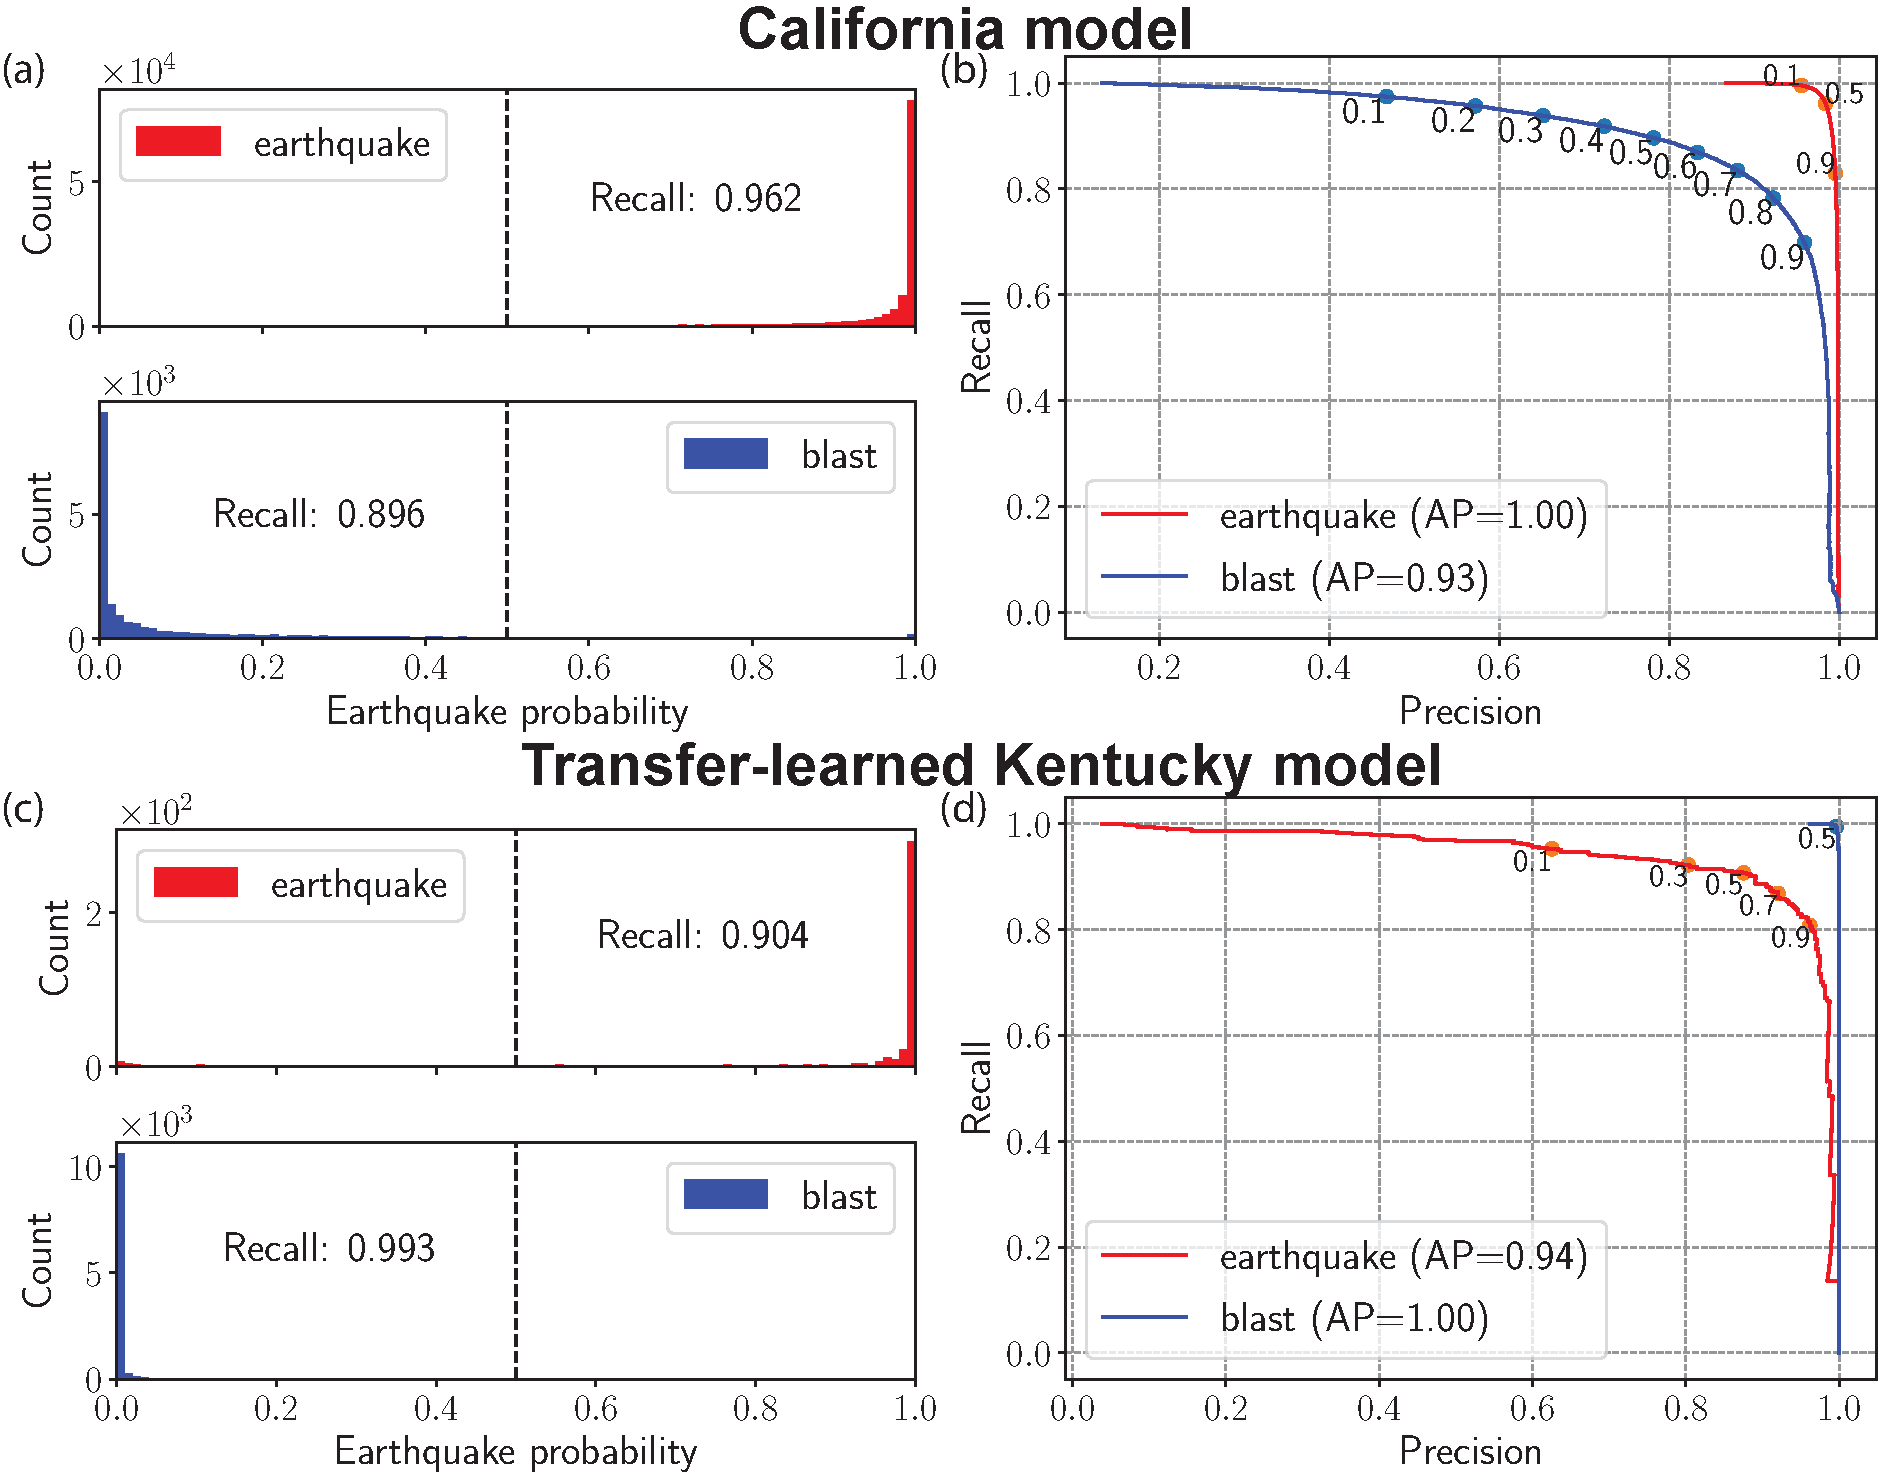
\includegraphics[width=.75\textwidth]{histogram.pdf}
\caption{Performances of (top panel) the California model and (bottom panel) the transfer-learned Kentucky model on respective test set. (a) Histograms of the single-station earthquake probability for earthquakes (red) and blasts (blue). The black dashed line marks the threshold of 0.5. (b) Precision-recall curves for earthquakes (red) and blasts (blue). AP, average precision. (c-d) Same as (a-b) except for the transfer-learned Kentucky model.}
\label{histogram}
\end{figure*}

We investigated the performance dependency on SNR, epicentral distance, magnitude and focal depth (Fig.~\ref{dependence}). The results show that recalls of both earthquakes and blasts increase with SNR, and decrease with epicentral distance, suggesting that signal quality is a major impact factor on classification accuracy. There is no link between the recall of earthquakes and magnitudes. There is a significant drop in the blast recall from \textgreater{95}\% to 66\% as the magnitude of blasts reaches \textit{M}2. There are two potential reasons for the drop: 1) the number of blasts in the bin of \textit{M} 2-3 is only 45 so that the estimated recall could be unstable; 2) only a few blasts have magnitudes \textgreater{2} so that our model does not learn well (Fig.~S2a). The recall of earthquakes slightly increases with depth, consistent with a previous finding that focal depth is an important discriminant \citep{koper,koper_20} given that most natural earthquakes are deeper than quarry blasts.

\begin{figure*}
\centering
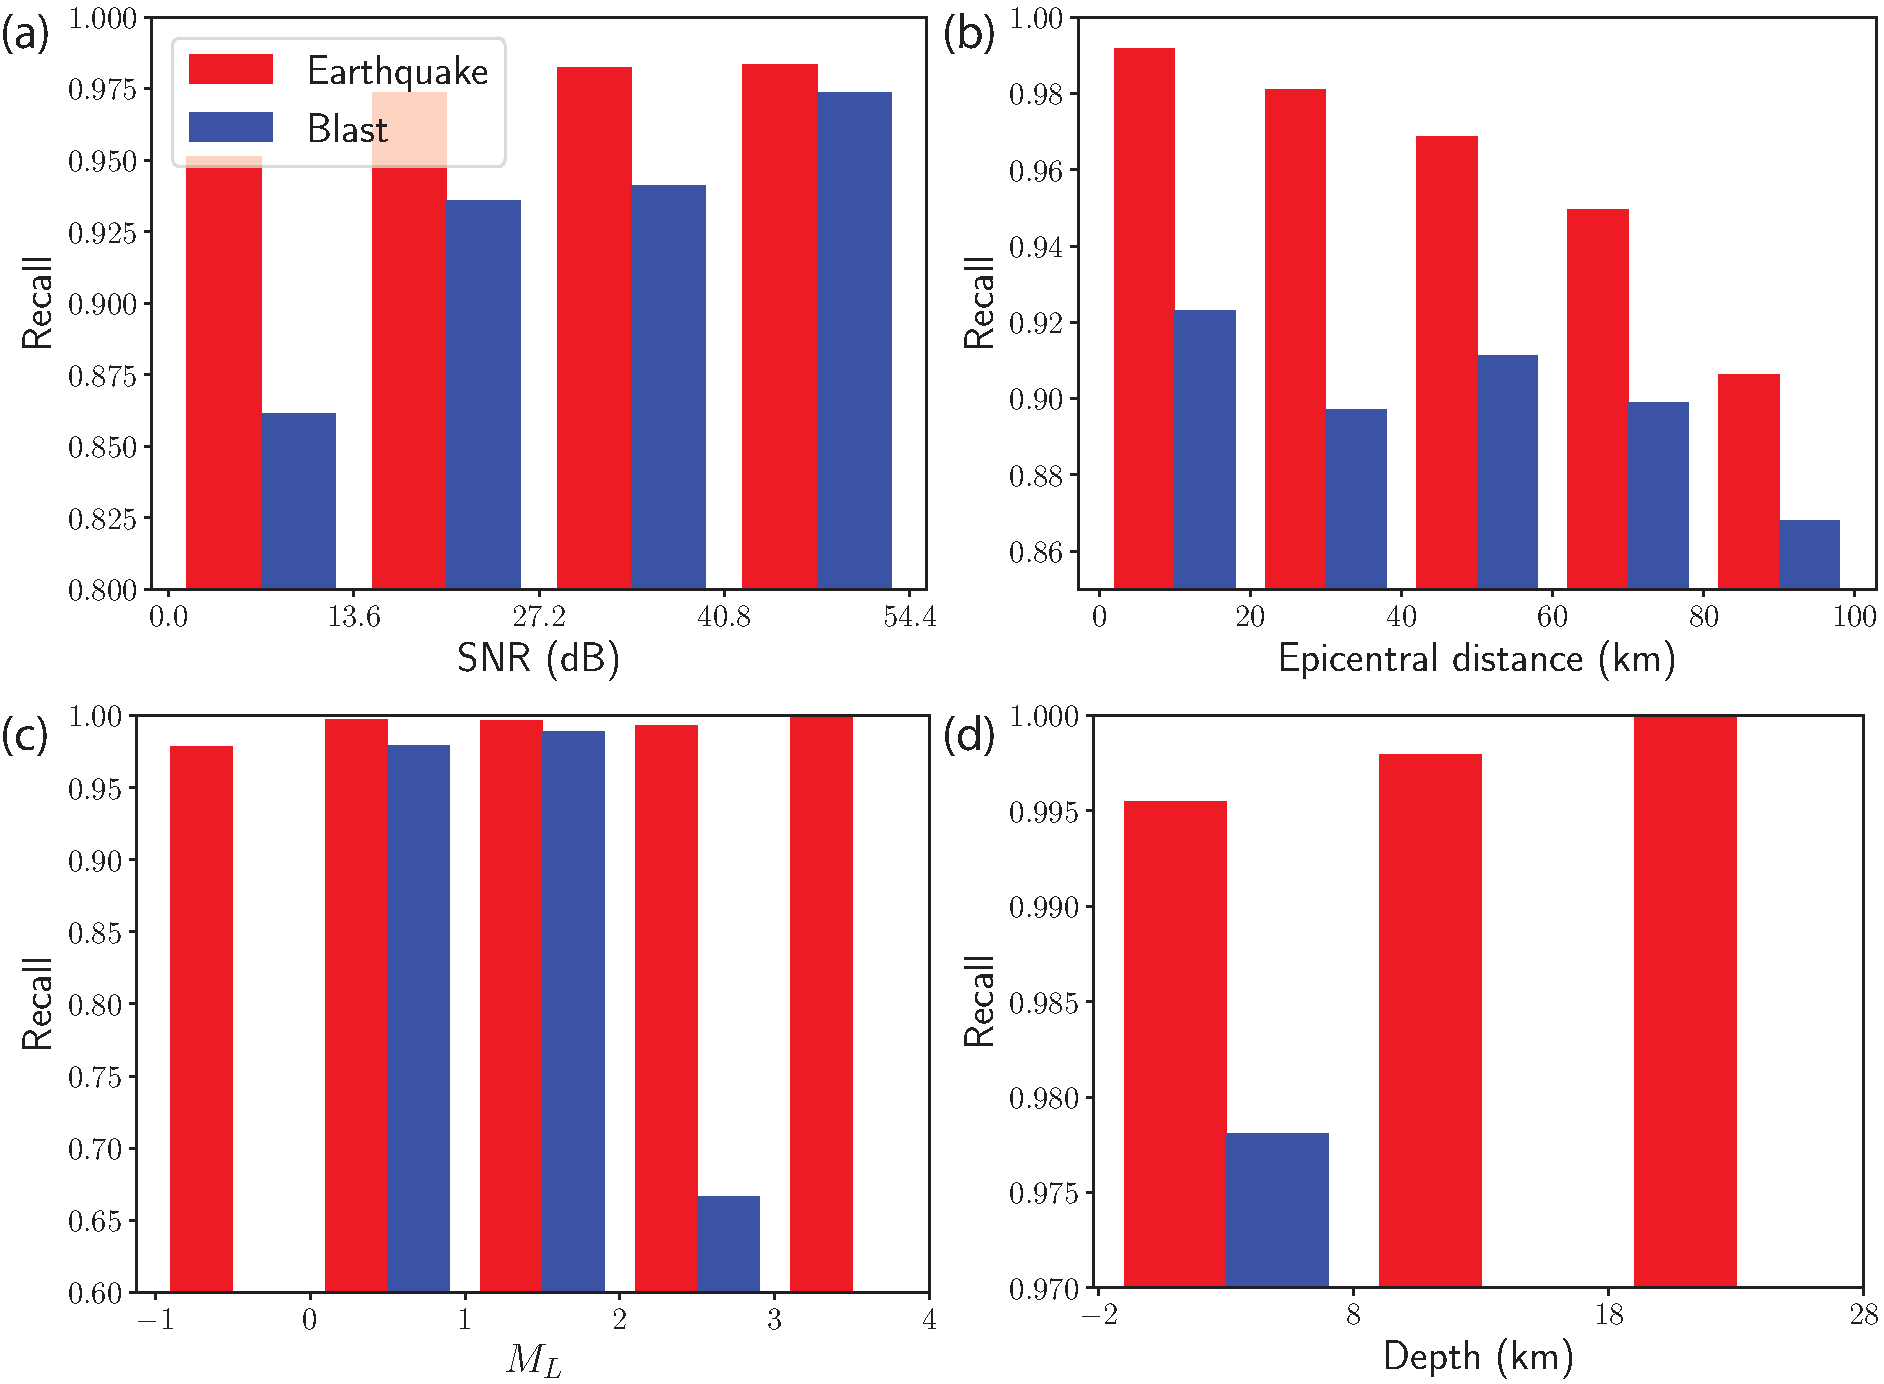
\includegraphics[width=.75\textwidth]{dependencce.pdf}
\caption{Variations of the recall of the California model on (a) SNR, (b) epicentral distance, (c) magnitude and (d) focal depth. Model recall is not shown if the number of samples in the bin is less than 15.}
\label{dependence}
\end{figure*}

\subsection{Transfer learning to eastern Kentucky}
We compared the performance of different strategies in eastern Kentucky:
\begin{enumerate}
\renewcommand{\theenumi}{(\arabic{enumi})}
\item Directly apply the California model to the Kentucky test set;
\item Re-train the model with the Kentucky data from scratch;
\item Fine-tune the model with the Kentucky data using two different strategies: fine-tuning and freezing.
\end{enumerate}

We explored the effects of random shifts on the performances of the re-trained and the transferred models. As previously mentioned, we have tested 1, 2, 4, 8, 16, and 27 random shifts for the earthquakes in Kentucky. Both the fine-tuning and the freezing strategy yield higher F1-scores than re-training (Fig.~\ref{repeated_times}). Besides, the performance seems to converge when waveform copies are more than 8. As 16 random shifts yield the best overall performance at the network and at the station level (Fig.~\ref{repeated_times}), hereafter we will only discuss the performances of the frozen and the re-trained model with 16 random shifts. We will refer to only the frozen model as the transfer-learned Kentucky model.

\begin{figure}
\centering
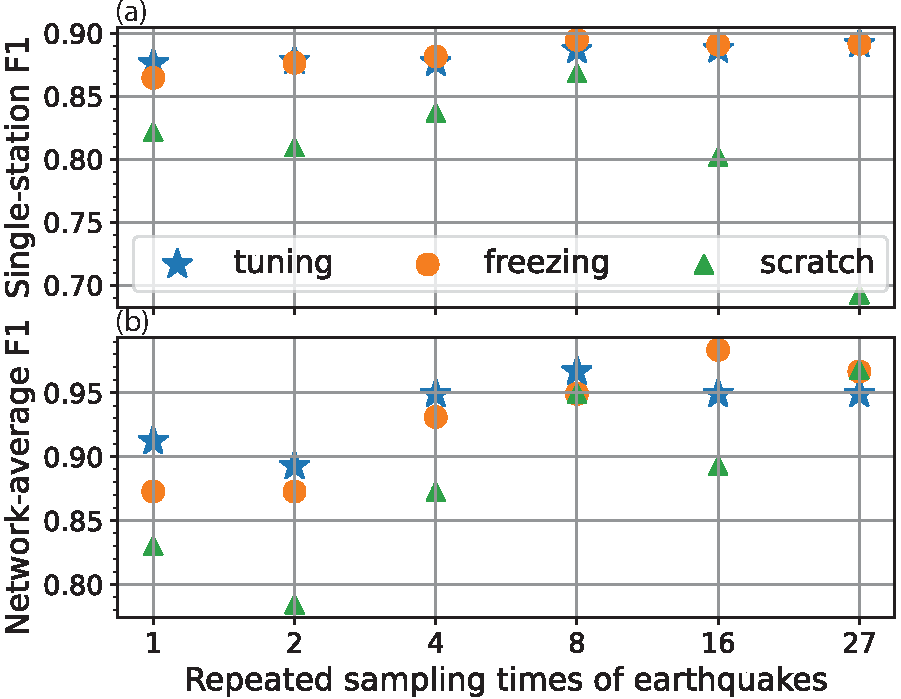
\includegraphics[width=.45\textwidth]{repeat_times.pdf}
\caption{Variations of the earthquake F1-score on the size of earthquake data and on the training strategies. As we increase the earthquake data size, (a) the F1-score estimated by single station slightly increases for fine-tuning and freezing; but it drastically fluctuates for re-training. (b) Same as (a) but the F1-score is estimated by network average.}
\label{repeated_times}
\end{figure}

Directly applying the California model to the Kentucky test set yields the lowest accuracy, the lowest earthquake precision and the lowest blast recall because of too many blasts misclassified as earthquakes (Table~\ref{performance_comparison}). The failure of this strategy further justifies the necessity of adjusting the original California model to fit the data in Kentucky. Moreover, removing the \textgreater{100}-km-epicentral-distance samples significantly increases the blast recall from 28.6\% to 63.6\% (Fig.~S5), indicating that the gap of epicentral distances between the two data sets is to blame for the degraded performance.

The re-trained model significantly outperforms the California model with the accuracy and the F1-score improved by 67.5\% and \textgreater{54.9}\%, respectively (Table~\ref{performance_comparison}). The transfer-learned model achieves the highest accuracy (99.0\%), the highest earthquake F1-score (86.9\%), and the highest blast F1-score (99.5\%) among the three models, demonstrating that the California model does provide additional knowledge to discriminate events in Kentucky. Compared to the re-trained model, the transfer-learned model increases the number of TNs from 326 to 403. Owing to the rise in TNs, the performance gain of the transfer-learned over the re-trained model is greater for earthquake than blast classification. 90.4\% of earthquake records and 99.3\% of blast records are correctly classified by the transfer-learned model (Table~\ref{socal_performance} and Fig.~\ref{histogram}c), with an AP of 0.94 for earthquakes and 1.0 for blasts (Fig.~\ref{histogram}d).

\begin{table*}
\caption{Performance comparison of three models in the eastern Kentucky dataset}
\label{performance_comparison}
\begin{tabular}{lcccccc}
\toprule[1pt]
Model&\multicolumn{2}{c}{Original California}&\multicolumn{2}{c}{Re-trained}&\multicolumn{2}{c}{Transfer-learned}\\
Accuracy&\multicolumn{2}{c}{0.310}&\multicolumn{2}{c}{0.985}&\multicolumn{2}{c}{\textbf{0.990}}\\
\hline
&Pred. EQ&Pred. QB&Pred. EQ&Pred. QB&Pred. EQ&Pred. QB\\
True EQ&417&29&326&120&403&43\\
True QB&8,227&3,288&68&11,447&78&11,437\\
Recall&\textbf{0.935}&0.286&0.731&\textbf{0.994}&0.904&0.993\\
Precision&0.048&0.991&0.827&0.990&\textbf{0.838}&\textbf{0.996}\\
F1-score&0.092&0.443&0.776&0.992&\textbf{0.869}&\textbf{0.995}\\
\bottomrule[1pt]
\end{tabular}
\end{table*}

\subsection{Model interpretation: Grad-CAM tests}
Although deep learning proves to be powerful in a wide range of applications, its decision-making process has been known for poor interpretability. As an end-to-end approach, CNNs do not provide direct clues on whether it truly identifies major seismic phases (e.g., \textit{P}, \textit{S} and coda) like human experts do. However, computer scientists have developed various techniques to shed light on the decision-making process of CNNs. We used the Grad-CAM test \citep{cam} to highlight the primary characteristics that the California model and the transfer-learned Kentucky model use to distinguish two signal types.

Specifically, Grad-CAM  visualizes the model sensitivity for each segment in the input seismograms. It first computes the gradients of either class’s score (or probability) with respect to the last convolutional layer’s output, i.e., the 256 feature maps in Fig.~\ref{cnn6}. These gradients reflect the relative contribution from each feature map to the score of the class of interest. Grad-CAM sums the absolute feature maps (1\texttimes{84} shape) with the gradients as weights, producing a weighted activation heatmap (1\texttimes{84}). The small-sized heatmap is then interpolated to the same size of the input seismogram (1\texttimes{5500}) to highlight which parts of the seismogram contribute more to the model output. More details about how to generate the heatmaps are detailed in Appendix~\ref{cam_appendix}.

\begin{figure*}
\centering
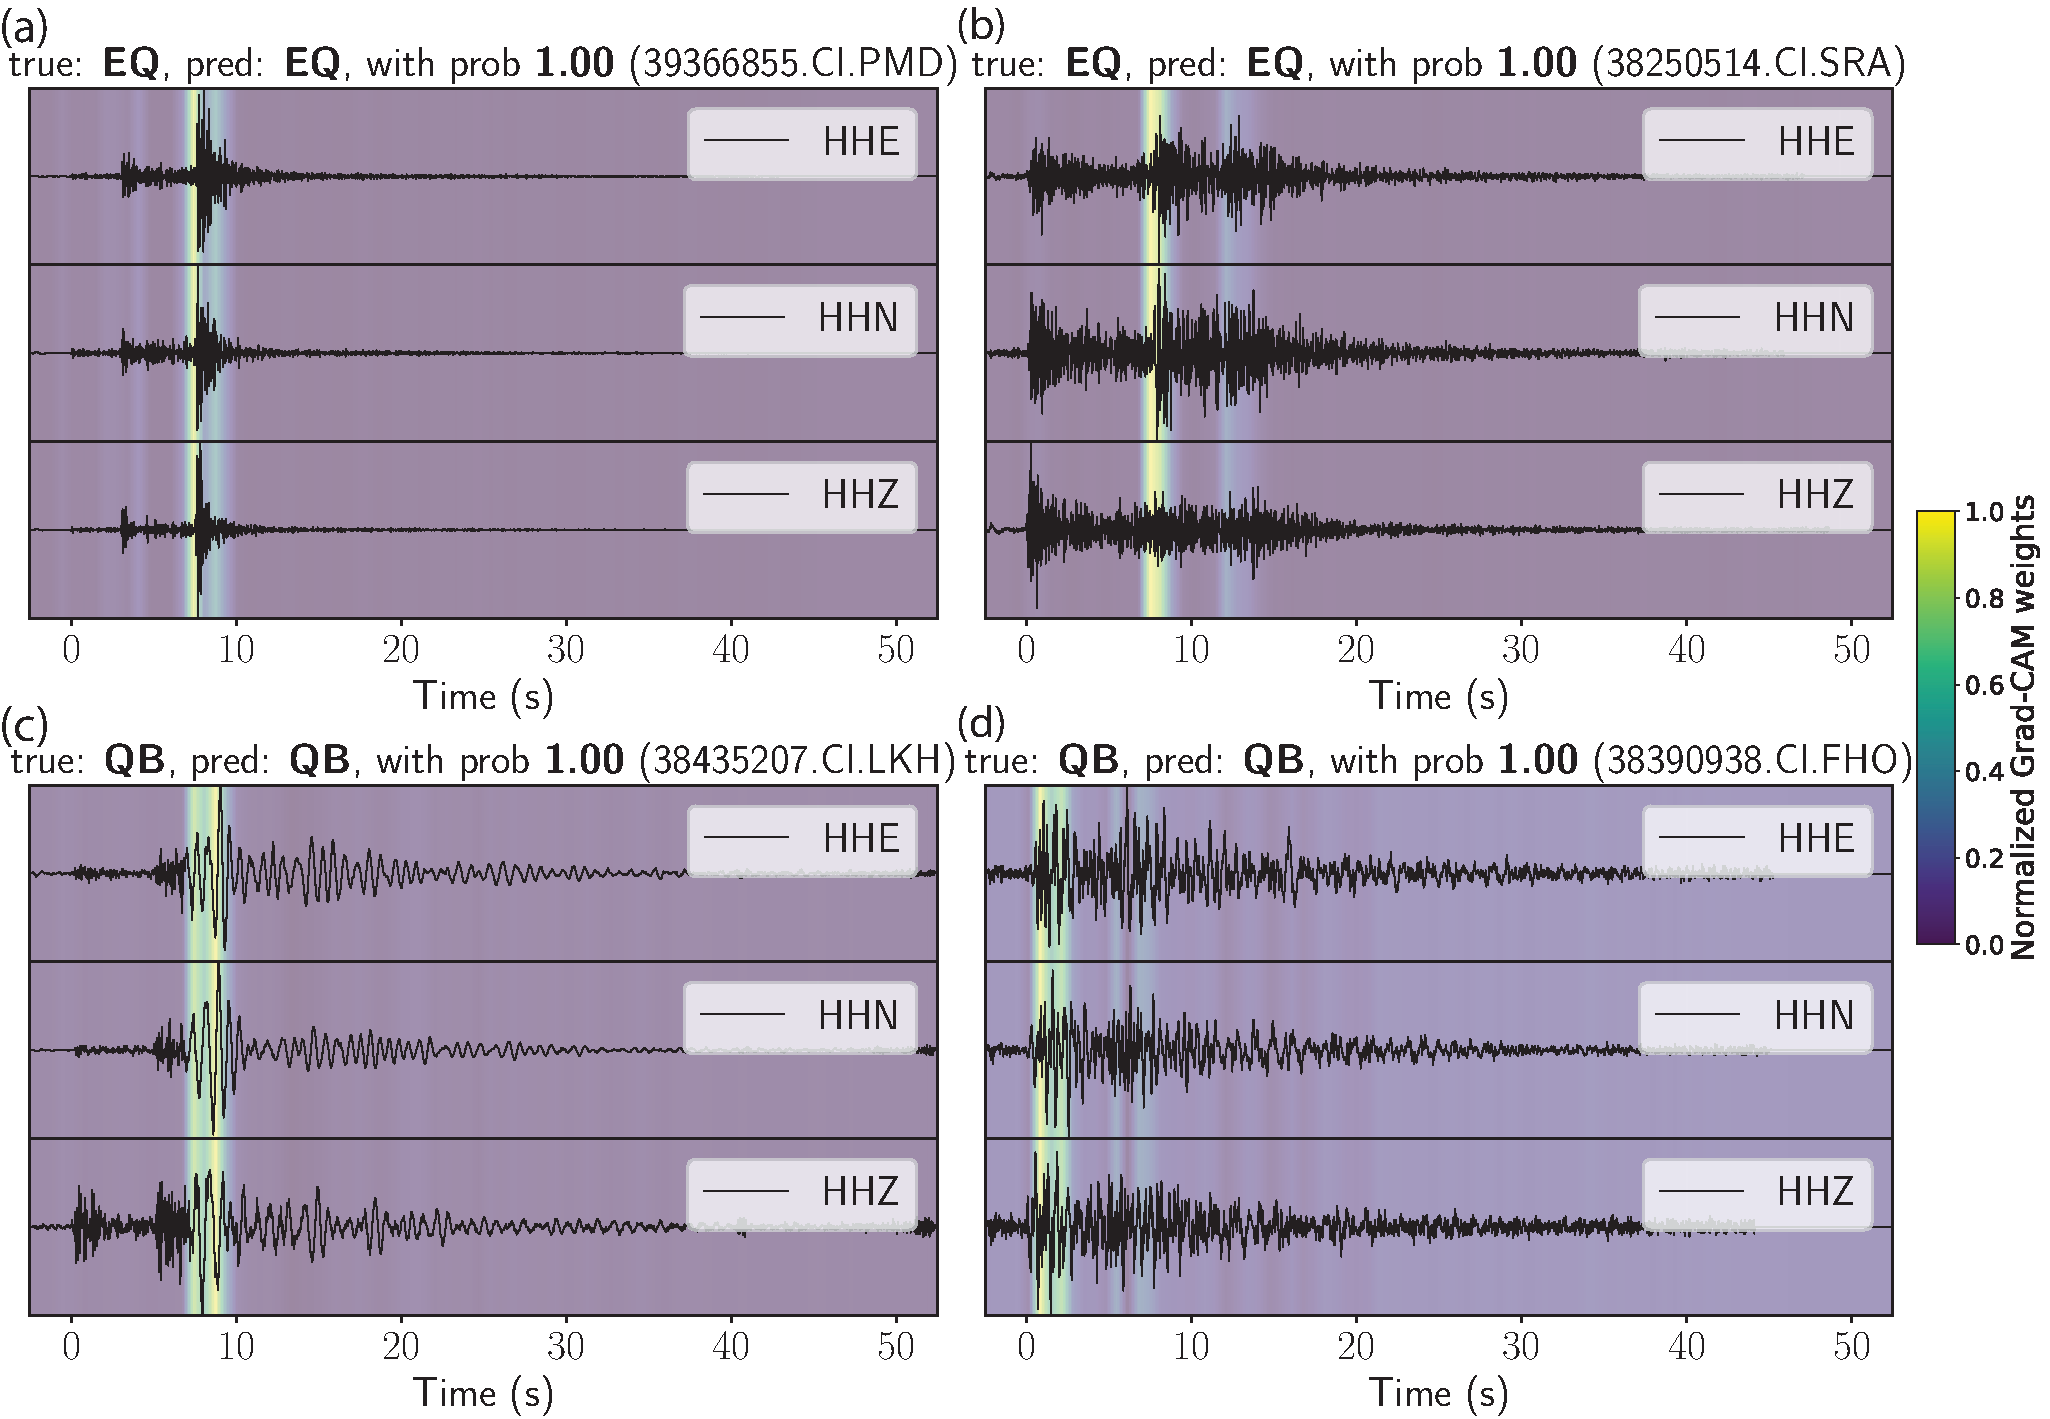
\includegraphics[width=.99\textwidth]{grad_CAM.pdf}
\caption{Grad-CAM tests for typical (a-b) earthquakes and (c-d) blasts in southern California. All traces are aligned by the \textit{P}-waves fixed at 0 s. The backgrounds are coloured by the normalized Grad-CAM weights. The probability for the predicted event type, the SCEDC event ID and station information are included in the plot titles.}
\label{cam}
\end{figure*}

\begin{figure*}
\centering
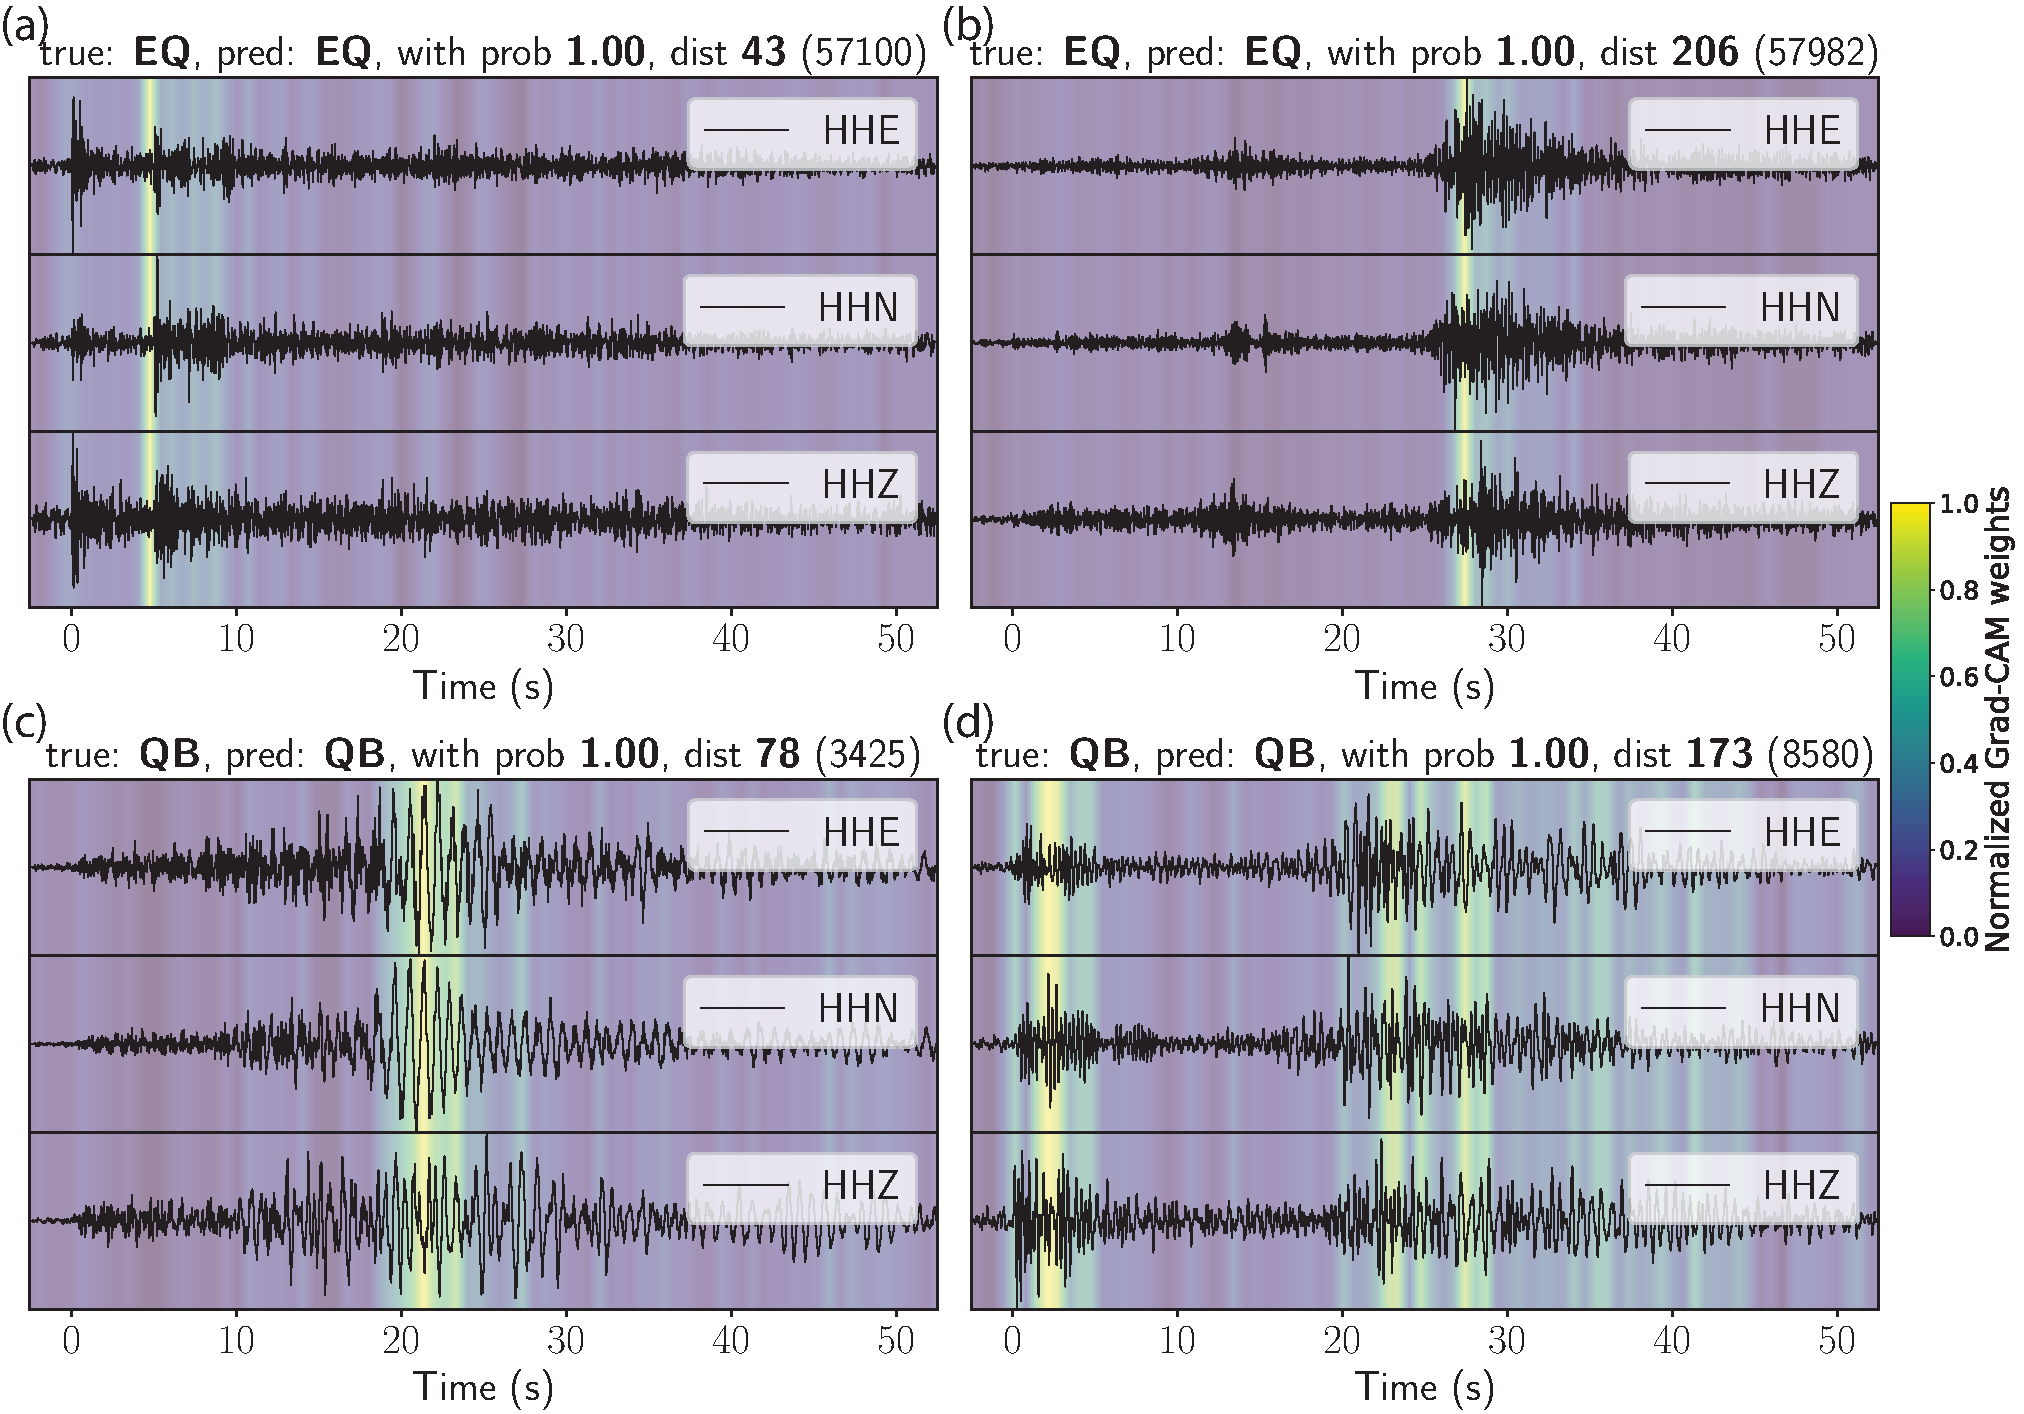
\includegraphics[width=.99\textwidth]{grad_CAM_ek.pdf}
\caption{Grad-CAM tests for typical (a-b) earthquakes and (c-d) blasts in eastern Kentucky, with the epicentral distance increasing from left to right. Symbols are the same as Fig.~\ref{cam}. The epicentral distances of the seismic records are also included in the plot titles (unit: km). The number in the parenthesis of plot titles is the index of record.}
\label{cam_ek}
\end{figure*}

Fig.~\ref{cam} shows the heatmaps (the backgrounds coloured by significance) and corresponding waveforms of four typical earthquakes and blasts in southern California. For earthquakes, our model pays the highest attention to the onset of \textit{S}-wave, with decreasing attention to the \textit{S} coda (Figs.~\ref{cam}a and \ref{cam}b). Comparatively, blasts' heatmaps have two distinct patterns. For the vast majority of blasts, our model focuses on the low-frequency \textit{S} coda (Fig.~\ref{cam}c) only. For a few blasts with weak to no \textit{S}-waves, our model shows an increasing emphasis on \textit{P}-waves and \textit{P} coda (Fig.~\ref{cam}d) accordingly. These results agree with previous observations that quarry blasts are relatively lacking in high frequency content \citep{allmann,korrat,kortstrom,su}. Particularly, quarry blasts in southern California are often characterized by long-duration and low-frequency \textit{S}-waves, a feature on which the SCSN analysts primarily relies to distinguish from local earthquakes (personal communication with Shang-Lin Chen).

Fig.~\ref{cam_ek} shows that the features used by the California model hold for Kentucky, even if the station is \textgreater{100} km far (Figs.~\ref{cam_ek}b and \ref{cam_ek}d). In addition, the features also hold for the mispredictions: the earthquake predicted as a blast has relatively weak \textit{S}-waves (Fig.~S6a) or low-frequency \textit{S} coda (Fig.~S6c); the blasts predicted as earthquakes have impulsive \textit{S} onsets (Figs.~S6b and S6d). In conclusion, Grad-CAM highlights the same diagnostic features for the same event types, suggesting that the model has learned consistent features of the earthquakes and blasts.

\section{Discussion and Conclusions}
We have developed two deep learning models to distinguish between local earthquakes and quarry blasts in southern California and in eastern Kentucky. The CNN model takes waveforms as direct input and automatically extracts implicit features that are optimized for classification. These models show generally high F1-score (\textgreater{83.5\%} on single station and \textgreater{96.7\%} by network average) for natural earthquakes and quarry blasts. Our results show that reliable classification can be achieved by using waveforms alone without source information. We find that although Kentucky has distinct data characteristics from California, transfer learning of the California model to eastern Kentucky still outperforms the retrained model. This demonstrates the efficacy of transfer learning in generalizing deep learning models across different regions.

\subsection{Comparison with previous methods}
\cite{allmann} proposed to use the misfit of \textit{P}-wave spectra to an $\omega^{-2}$ source model as a discriminant between local earthquakes and blasts in southern California. They examined the events recorded by at least three stations with SNR \textgreater3 dB on three frequency bands, and reported a nearly 90\% classification accuracy (i.e., 90\% of earthquakes and nearly 90\% of blasts were correctly classified at the network level). Comparatively, our California model achieves overall 99.3\% accuracy (i.e., 99.7\% of earthquakes and 97.7\% of blasts are correctly classified at the network level, Table~\ref{socal_performance}) on a much larger data set, with a looser data selection criterion and simpler preprocessing.

In eastern Kentucky, \cite{miao} carefully designed multiwindow spectral features  and trained a two-layer artificial neural network that achieved an AP of 0.8558$\pm$0.0235 for earthquakes. Taking into account the trade-off between model complexity and accuracy (Fig.~S7), we use a deep model with six convolutional layers to automatically extract the features and achieve a higher AP of 0.94 for earthquakes. Also, our model yields higher F1-scores for earthquakes (0.869) and for blasts (0.995) than those by \cite{miao} (0.3526$\pm$0.0712 for earthquakes, 0.9854$\pm$0.0051 for blasts). Different from the test set of \cite{miao} which includes the events occurring between 2015 and 2019, our test set contains only those latter events occurring between 2018 and 2019 (Table~\ref{division}). Such data splitting strategy makes the estimations for our model closer to the model's true performances in realistic monitoring conditions \citep{linville_19}. Although the simpler model by \cite{miao} indicates that the carefully handcrafted features may reduce the need of complex models, our approach is potentially more generalizable to other regions as our model can be automatically fine-tuned (i.e., fine-tuning or freezing) and requires little expert knowledge.

Without handcrafted features, the deep learning models proposed by \cite{linville_19} also automatically distinguish between mining blasts and tectonic earthquakes in Utah. \cite{tibi_compare} compared the models to amplitude-ratio-based methods and concluded that deep learning methods are generally more robust for low-SNR events. Our CNN models differ from \citeauthor{linville_19}’s in input data formats and data balancing. First, they used the spectrograms of three-component waveforms which are rotated to radial, transverse and vertical directions. We did not rotate the waveforms in order to work without knowing the exact locations. Second, the number of earthquakes and blasts are more balanced in Utah \citep{linville_19,tibi_compare}, compared to the extreme class imbalance in southern California and eastern Kentucky. Thus, we used data augmentation to mitigate class imbalance. In our study, different dominant classes of the two datasets also offer us an opportunity to test the effectiveness of transfer learning.

Using four well-calibrated data sets \citep{wang_grl}, \cite{kong} robustly classified between earthquakes and explosions with physics-based features (i.e., the phase ratio of \textit{P}-to-\textit{S} and the magnitude difference of $M_L$-$M_C$). They reported that the inclusion of the physics-based features improves the generalizability of their deep learning models across diverse tectonic settings, despite the features might be unavailable in presence of strong noise. They also used Grad-CAM heatmaps to show what their model has learned. Our finding that the low-frequency \textit{S} coda is of great importance to blasts is consistent with fig.~3 in \cite{kong}. However, the most important feature for their explosions seems always to be \textit{P}-waves, likely due to a higher SNR threshold (3 dB) for \textit{P}-waves used in their study.

\subsection{Practical considerations in deep learning strategies}
We designed our models to take input with minimal preprocessing for more generalizability and ease of use. For this consideration, conventional preprocessing operations including spectrogram calculation and component rotation were both skipped. Possibly, the model performance could be further enhanced if some of preprocessing operations are applied to enhance signal quality. However, minimal human interference of the data can reduce on-line runtime and offer flexibility to transfer the models to other regions. Our model can classify 1,600 samples within 1 second during on-line testing, and the model file is as small as 0.5 Mb. The fast-processing speed and small file size enable easy integration of the models into real-time seismic monitoring systems.

Class imbalance is a major problem in the classification for both California and Kentucky, where different treatments can lead to different results. In the California case, training without upsampling blast data produces a lower recall of 72.9\% for blasts. Besides upsampling the minority class, we tested two other strategies, i.e., downsampling the majority class and cost-sensitive learning \citep{cost_sensitive}, to improve the performance. Compared with upsampling, downsampling reduces both quantity and diversity of the training data and the F1-score drops by 1.1\% and 12.1\% for earthquakes and blasts, respectively. As for cost-sensitive learning, we increased the weight of the loss term for the minority class, i.e., misclassifying blasts as earthquakes is penalized more than misclassifying earthquakes as blasts. However, cost-sensitive learning yields only a recall of 83.0\% for blasts, as compared to a recall of 89.6\% for blasts with upsampling. Thereby, upsampling appears more effective to mitigate the imbalance problem, likely because various versions of time shifts together with the basic seismic data augmentations (Appendix.~\ref{data_aug}) increase the overall data diversity. Nonetheless, even with upsampling, the minority class (i.e., blasts in southern California, earthquakes in eastern Kentucky) inevitably tends to have a lower precision and F1-score because the increased data diversity is still limited for the minority class.

Finally, the input window length also affects the performance. We have tested a window length of 35 s. Compared to the 55-s window, the 35-s window yields a better performance in southern California (95.4\% accuracy) but a worse performance in eastern Kentucky (98.3\% accuracy) than the window length of 55 s. This is likely a combined result of the longer source-receiver distance (mostly \textgreater100 km), the longer \textit{P}\slash \textit{S} separation, and the longer \textit{P}\slash \textit{S} coda in Kentucky. The longer coda could result from the lower seismic attenuation in eastern Kentucky than southern California \citep{attenu_ek,attenu_socal}.

\subsection{Suggestions for further use}
Although our deep learning models produce generally reliable results, there remains room for improvement given that some waveforms were misclassified. We re-evaluated the misclassified events based on waveforms, first-motion polarities, origin time, spatial clustering and focal depths. Of the 51 misclassified events in the California test set (Table~\ref{socal_performance}), 16 (Table~S2, Figs.~S8 and S9) were likely mislabelled by SCSN analysts. Fig.~\ref{mislabel} shows an earthquake and a blast misclassified on almost all stations, which were likely falsely labelled. Removing the mislabelled events from the test set results in an increase in the F1-score of earthquakes and blasts, 0.13\% and 0.56\%, respectively. For the Kentucky test set, there are only two mispredictions, i.e., the Event 1 and 2 in Fig.~\ref{map_ek} (Table~\ref{socal_performance}). Both events occur at night so neither of them are blasts. The Event 1 is unlike typical earthquakes as most of its \textit{P}- and \textit{S}-waves are emergent rather than impulsive (Fig.~\ref{mislabel_ek}a). Due to its emergent \textit{P}-waves with extended coda, it is likely an induced earthquake \citep{miao}. As to the Event 2, we have confirmed that it was falsely labelled (Fig.~\ref{mislabel_ek}b). In addition to the mislabels, path and site effects can significantly alter the waveforms and result in potential misclassification. Averaging the probabilities of multi-station recordings can help mitigate the misclassification caused by the variations of path and site effects. Compared to single-station classification, network-averaged classification improves the F1-scores by \textgreater{2.3}\% in the California case, \textgreater{0.4}\% in the Kentucky case. More specifically, network average greatly improves the minority class’s F1-score (an increase of 15\% in F1-score for blasts in California, 10\% for earthquakes in Kentucky). The larger impact of network average on the California than the Kentucky test set is likely because 
each event has generally more available stations in California than in Kentucky (Fig.~S10). More stations for a single event can help stabilize the final prediction. Similarly, majority voting, which simply counts the output classes of all stations, may improve performance at the network level \citep{liu}. It is worth noting that both network average and majority voting require that phase association has been done. One may argue that after phase association, event depth can help seismic analysts classify between deeper earthquakes and shallower blasts. However, the depth discriminant fails (Fig.~S11a) if the reported depth of an earthquake is as shallow as a blast, or if the reported depth of a blast is falsely deep (Fig.~S12) due to poor station coverage. Compared to the blurred decision boundary drawn by the focal depth (Fig.~S11a), the network-averaged probability is a much more robust discriminant (Fig.~S11b) enabling identification of the mislabels in historical seismic catalogues. Finally, in real-time operation, there might be events neither natural earthquakes nor quarry blasts. For example, mining-induced earthquakes might be similar to both earthquakes and blasts as their source mechanisms can be double-couple, isotropic, or a combination of both \citep{koper}. Including other classes of events to further reduce ambiguity remains a subject of future work.

\begin{figure*}
\centering
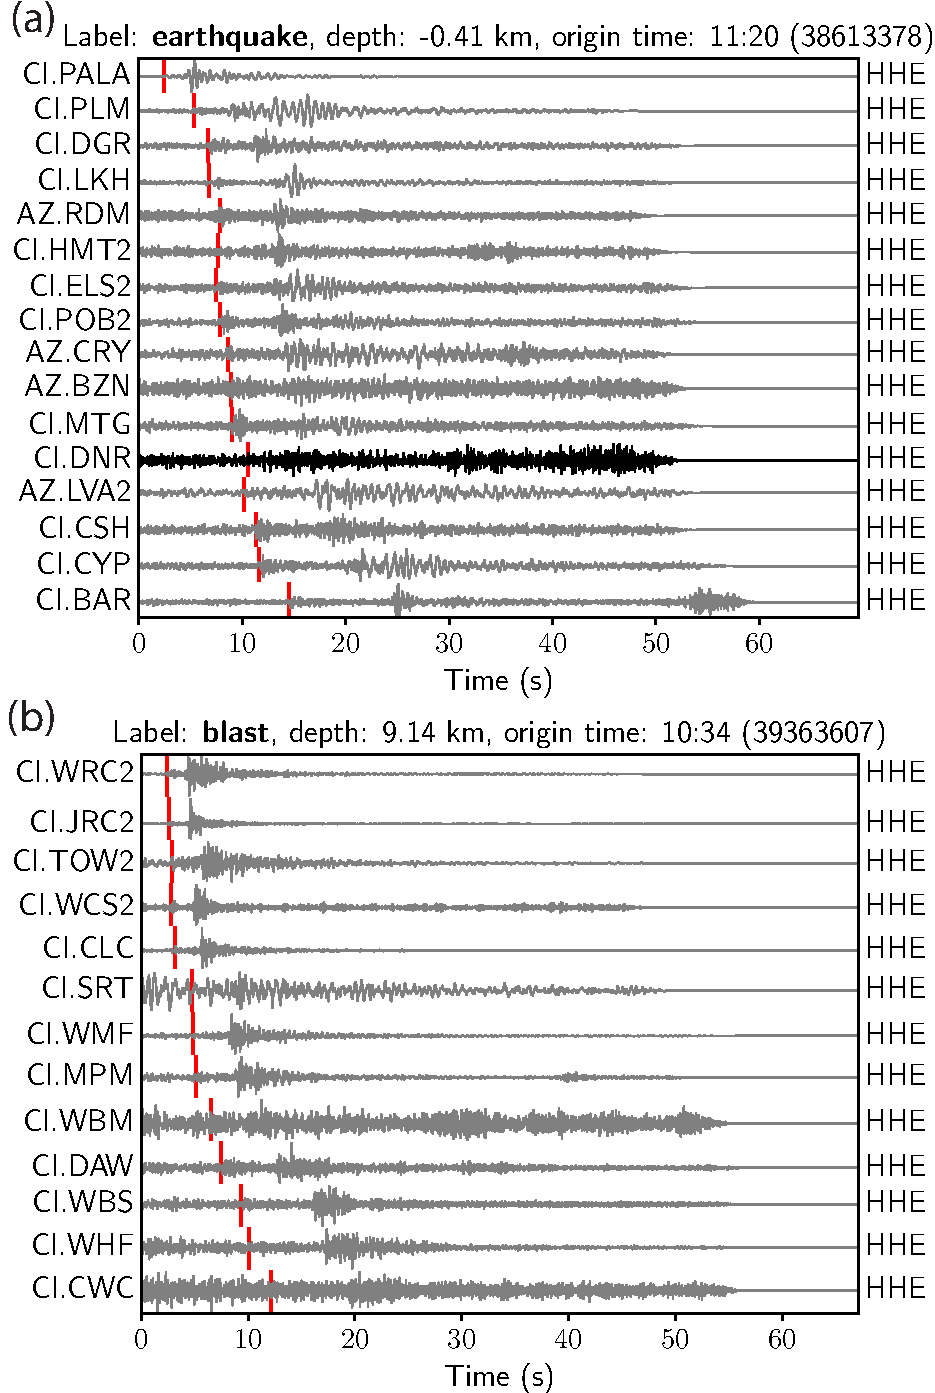
\includegraphics[width=.8\textwidth]{mislabelling.pdf}
\caption{Example of two events in southern California potentially mislabeled in the SCSN catalogue. (a) An earthquake (SCEDC event ID 38613378) classified as a blast on almost all stations (grey) except CI.DNR (black). All traces are aligned by the origin time, with \textit{P}-wave arrival times marked by the red lines. Notice that the reported depth and the origin time of this event are -0.41 km and 11:20 AM (California's local time), respectively. This event (the red star in Fig.~\ref{map}) occurs within a blast cluster, indicating that it is likely a blast but falsely labelled. (b) A quarry blast classified as an earthquake on all stations (grey). This event (the blue star in Fig.~\ref{map}) occurs within a cluster including both earthquakes and blasts. Its reported depth 9.14 km is well beyond the depth range of typical blasts.}
\label{mislabel}
\end{figure*}

\begin{figure*}
\centering
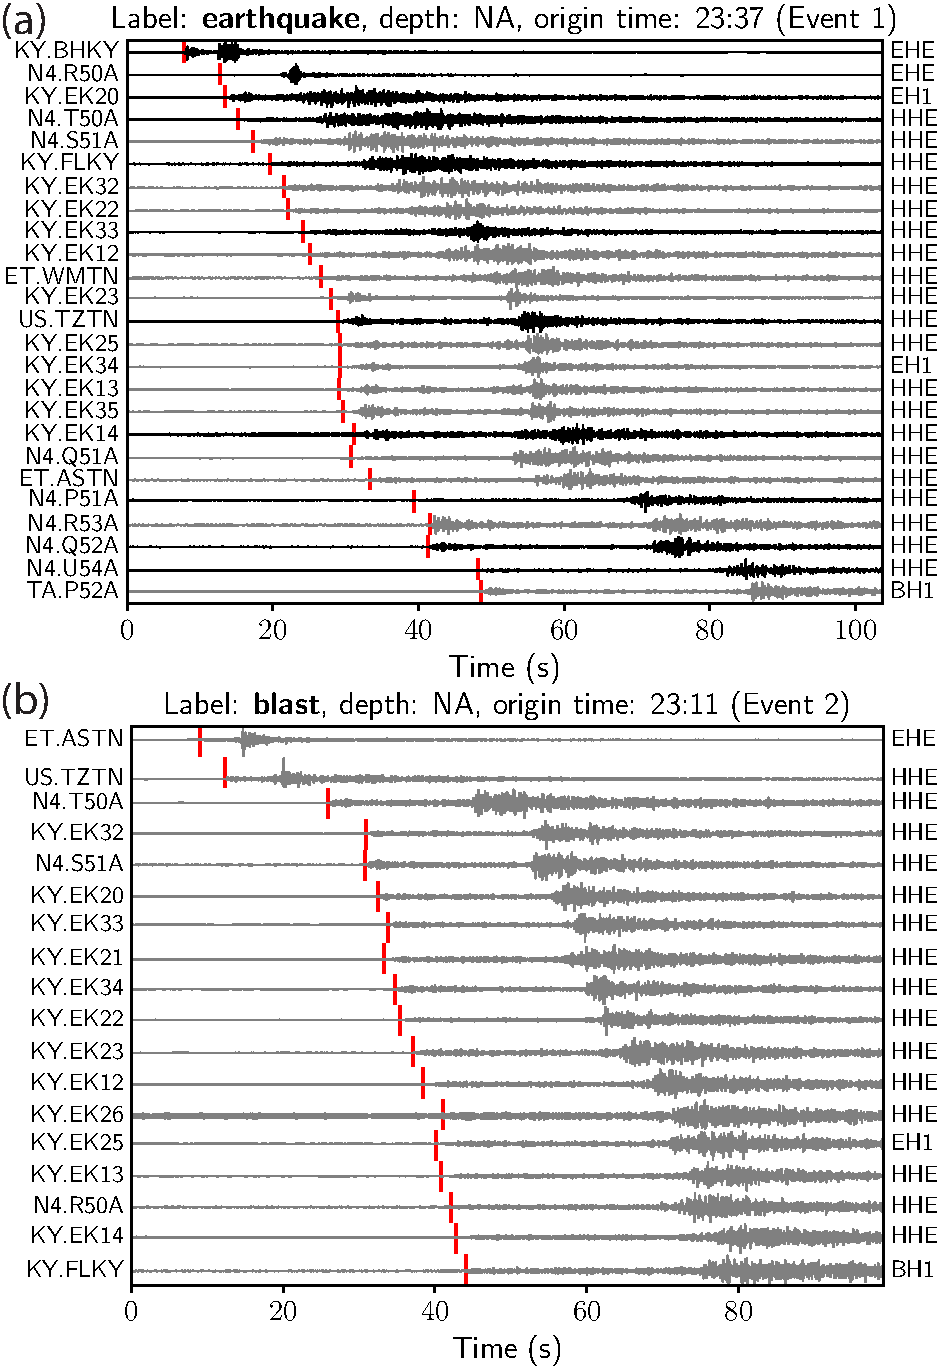
\includegraphics[width=.85\textwidth]{mislabelling_ek.pdf}
\caption{Waveforms of the only two mispredictions made by the transfer-learned Kentucky model at the network level (Table~\ref{socal_performance}). Annotations and colours follow Fig.~\ref{mislabel}. NA, not available. Both Event 1 (the red star in Fig.~\ref{map_ek}) and Event 2 (the blue star in Fig.~\ref{map_ek}) occur at night without blasting clusters nearby, confirming they are not blasts. Hence, at least Event 2 is falsely labelled.}
\label{mislabel_ek}
\end{figure*}

As different areas seem to have different characteristics of blasts and earthquakes, when applying our classification models to other areas, we strongly recommend using the transfer learning strategy. We have shown that transfer learning is the best solution among the three strategies for the eastern Kentucky case. Although deep learning models are increasingly used in seismology and many efforts have been made to pursue a universal model that works best for all data \citep{gpd,phasenet,mousavi}, we argue that rather than pursuing an optimal universal model, customizing models that work optimally for specific regions is probably a more viable pathway. With the help of transfer learning, regions with short seismic monitoring histories could have high-quality deep learning models comparable to those in well-instrumented regions at an economical price. 

\begin{acknowledgments}
We thank the editor and two anonymous reviewers for their insightful and helpful comments to improve this article. We thank the Southern California Seismic Network and the Kentucky Seismic and Strong-Motion Network for providing seismic data. JZ thanks Shang-Lin Chen for email communication on how seismic events are classified by SCSN analysts. This research was supported by the National Key R\&D Program of China (No. 2021YFC3000700 and 2022YFC3005602), the National Natural Science Foundation of China (No. 42274063 and 41974044) and the Special Fund of the Institute of Geophysics, China Earthquake Administration (No. DQJB21Z05).
\end{acknowledgments}

\begin{dataavailability}
\label{data_avai}
Seismic waveforms and catalogues used in the California study are from the Southern California Earthquake Data Center (doi: \url{10.7909/C3WD3XH1}). Some empirical rules to discriminate earthquakes and blasts, adopted by the SCSN analysts, are available at \url{https://www.scsn.org/index.php/education-outreach-2/understanding-waveforms/index.html}. The pure noise used for data augmentation is from the STanford EArthquake Dataset (STEAD, available at \url{https://github.com/smousavi05/STEAD}). The temporary network EKMMP used in Kentucky is a part of the Kentucky Seismic and Strong Motion Network (doi: \url{http://dx.doi.org/10.7914/SN/KY}). The regional network N4 (\url{https://www.fdsn.org/networks/detail/N4/}), ET (\url{https://www.fdsn.org/networks/detail/ET/}) and NM (\url{https://www.fdsn.org/networks/detail/NM/}), USArray Transportable Array TA (\url{https://www.fdsn.org/networks/detail/TA/}) data are available at IRIS DMC (\url{https://ds.iris.edu/mda/N4/}, \url{https://ds.iris.edu/mda/ET/}, \url{https://ds.iris.edu/mda/NM/}, \url{https://ds.iris.edu/mda/TA/}). The Earthworm software package is available at \url{www.isti.com/products/earthworm}.
\end{dataavailability}

\bibliographystyle{gji}
\bibliography{manuscript}

\section*{SUPPORTING INFORMATION}
\textbf{Figure~S1}. Seismic stations in the California data set, coloured by different networks.\\
\textbf{Figure~S2}. Histograms of (a) magnitude, (b) depth, (c) epicentral distance and (d) SNR of the California data set.\\
\textbf{Figure~S3}. Seismic stations in the Kentucky data set. Note that EKMMP, abbreviated as EK, is a part of the temporary Eastern Kentucky Microseismic Monitoring Network.\\
\textbf{Figure~S4}. Histograms of (a) magnitude, (b) depth, (c) epicentral distance and (d) SNR of the Kentucky data set. The magnitude and depth of the blasts are not available.\\
\textbf{Figure~S5}. The performances of the original California model on the Kentucky test set. (a) Histograms of the earthquake probabilities, predicted by the California model, for the entire Kentucky test set. (b) Same as (a) but the samples with \textgreater{100}-km epicentral distances have been removed.\\
\textbf{Figure~S6}. Grad-CAM tests for four mispredictions in (a-b) southern California and (c-d) eastern Kentucky. Symbols are similar to those in Figs. 8 and 9.\\
\textbf{Figure~S7}. Trade-off between model complexity and accuracy.\\
\textbf{Figure~S8}. Distribution of false positives and potential mislabels in the California test set. The red and the blue dots are earthquakes and blasts labelled by SCSN analysts. The circles and the star mark 20 false positives colour-coded by event depth, among which 7 are potential mislabels annotated by corresponding SCEDC event IDs and listed in Table S2.\\
\textbf{Figure~S9}. Distribution of false negatives and potential mislabels in the California test set. Symbols are similar to those in Fig.~S8.\\
\textbf{Figure~S10}. Probability density functions of the number of available stations for the test events in Kentucky (blue) and California (orange). Each test event has 13 stations on average in Kentucky and 21 in California.\\
\textbf{Figure~S11}. Event classification according to (a) depth and (b) network-averaged earthquake probability for the California test set. (a) With 2 km as the depth threshold (black dashed line), the recalls for earthquakes and blasts are 92.0\% and 90.3\%, respectively. The recalls for a deeper threshold (3 km, grey dashed line) are shown in grey. (b) With 0.5 as a probability threshold (black dashed line), 99.7\% of the earthquakes and 97.7\% of the blasts are correctly classified.\\
\textbf{Figure~S12}. Examples of the anomalously ``deep'' events.\\
\textbf{Table~S1}. Hyperparameters for model training\\
\textbf{Table~S2}. Potential mislabels in the California test set\\

\appendix
\section{Definition of SNR}
\begin{equation}
\label{snr}
SNR=10\times\log{\frac{P_{signal}}{P_{noise}}},\\
P_s=\sum_{i=1}^{500}(s[i]-\overline{s})^2
\end{equation}
, where $P_{signal}$ and $P_{noise}$ are the power of 5 s signal after and the 5 s noise before the \textit{P}-wave arrival, respectively; $\overline{s}$ is the average amplitude of the 5 s waveform.

\section{Basic seismic data augmentations}
\label{data_aug}
Data augmentations are implemented on the fly so that our model sees a new version of the training set at every epoch. We augment the waveforms with SNR \textgreater{1} dB and keep the rest unchanged. Four augmentation methods are used: channel dropout (i.e., randomly dropping one or two of the three components); adding data
gaps (i.e., filling zeros to a random waveform segment \textless{11} s); waveform clipping (i.e., reducing the dynamic range of the waveform by a random level of \textless{50}\%) and superimposing noise to the filtered waveforms with amplitude ratio \textless{0.2}. We randomly choose one of the four methods to alter every sample with a probability. The probabilities for the four methods are 0.3, 0.2, 0.3 and 0.5, respectively.

\section{Gradient-weighted class activation mapping}
\label{cam_appendix}
Many works have proved that the last convolutional layer of CNN models strikes a balance between extracting high-level semantic features and retaining detailed spatial information. That's why Grad-CAM \citep{cam} used the output of the last convolutional layer i.e., the 256 feature maps in Fig.~\ref{cnn6}, to visualize the relative importance of each waveform segments. To this end, we first stacked all 256 feature maps with the weights defined by eq.~\ref{weight}.
\begin{equation}
\label{weight}
\alpha_k^c=\frac{1}{84}\sum_{i=1}^{84}\frac{\partial y^c}{\partial A_i^k}
\end{equation}
, where $\alpha_k^c$ represents the gradient of the score $y^c$ for class $c$, with respect to the $k$-th feature map, $A^k$; $i$ is the index of features.
After stacking, we applied a ReLU activation function to the stacked map (eq.~\ref{stack}). The ReLU activation function supresses negative influences thus only those segments with positive influences on the score $y^c$ are highlighted.
\begin{equation}
\label{stack}
L_{Grad-CAM}^c=ReLU(\sum_{k=1}^{256}\alpha_k^cA^k)
\end{equation}
Finally, the derived class-specific activation map was up-sampled to the input seismograph resolution using bilinear interpolation to form the final heatmap.

\label{lastpage}

\end{document}